\documentclass[11pt]{article}
\usepackage[margin=1in]{geometry}
\usepackage{newtxtext,newtxmath}
\usepackage{microtype}
\usepackage{placeins}
\usepackage{booktabs}
\usepackage{graphicx}
\usepackage{amsmath}
\usepackage{tikz}
\usetikzlibrary{arrows.meta,positioning,shapes.geometric,calc,fit,backgrounds}
\usepackage[hidelinks]{hyperref}
\usepackage[capitalise,noabbrev]{cleveref}
\usepackage{xcolor}
\definecolor{accent}{RGB}{27,120,120}
\definecolor{dimmed}{RGB}{120,120,120}
% Shared TikZ styles for the LazyCode paper figures.
% Convention (load-bearing, see sec:implementation):
%   accent  = SHIPPED, load-bearing code today
%   dimmed  = DESIGNED / plumbed only, not reachable at runtime
\usetikzlibrary{arrows.meta,positioning,shapes.geometric,calc,fit,backgrounds,
                decorations.pathreplacing,decorations.pathmorphing,patterns}

\definecolor{danger}{RGB}{160,60,45}
\definecolor{inkgray}{RGB}{70,70,70}

\tikzset{
  % ---- shipped ----------------------------------------------------------
  box/.style={
    rounded corners=2pt, draw=accent, line width=0.6pt,
    fill=accent!6, text=black,
    font=\sffamily\footnotesize, align=center,
    inner xsep=4pt, inner ysep=3.5pt, minimum height=8mm},
  boxs/.style={box, font=\sffamily\scriptsize},
  % emphatic (event log, contracts)
  boxf/.style={box, fill=accent!14, line width=0.8pt},
  % neutral / input-output terminals
  term/.style={
    rounded corners=5pt, draw=inkgray, line width=0.6pt, fill=white,
    font=\sffamily\footnotesize, align=center,
    inner xsep=4pt, inner ysep=3.5pt, minimum height=7mm},
  % ---- designed only ----------------------------------------------------
  dbox/.style={
    rounded corners=2pt, draw=dimmed, line width=0.5pt, dash pattern=on 2pt off 1.6pt,
    fill=dimmed!7, text=dimmed,
    font=\sffamily\footnotesize, align=center,
    inner xsep=4pt, inner ysep=3.5pt, minimum height=8mm},
  dboxs/.style={dbox, font=\sffamily\scriptsize},
  % ---- containers -------------------------------------------------------
  group/.style={
    rounded corners=3pt, draw=inkgray!45, line width=0.5pt,
    dash pattern=on 3pt off 2pt, inner sep=5pt},
  % ---- arrows -----------------------------------------------------------
  ar/.style={-{Stealth[length=1.9mm,width=1.5mm]}, draw=accent, line width=0.6pt},
  arg/.style={-{Stealth[length=1.9mm,width=1.5mm]}, draw=inkgray, line width=0.6pt},
  dar/.style={-{Stealth[length=1.9mm,width=1.5mm]}, draw=dimmed, line width=0.5pt,
              dash pattern=on 2pt off 1.6pt},
  % ---- labels -----------------------------------------------------------
  lbl/.style={font=\sffamily\scriptsize, text=inkgray, align=center, inner sep=1.5pt},
  lbls/.style={font=\sffamily\fontsize{6}{7}\selectfont, text=inkgray,
               align=center, inner sep=1.2pt},
  dlbl/.style={font=\sffamily\scriptsize, text=dimmed, align=center, inner sep=1.5pt},
  wtag/.style={font=\sffamily\bfseries\scriptsize, text=danger, inner sep=1.2pt},
  banner/.style={font=\sffamily\bfseries\scriptsize, text=accent, align=left},
}

% small gray annotation text inside a node
\newcommand{\lbltext}[1]{{\sffamily\scriptsize\color{inkgray}#1}}
\newcommand{\lbltiny}[1]{{\sffamily\fontsize{6}{7}\selectfont\color{inkgray}#1}}


\title{\textbf{LazyCode: Compiling Interactive Intent into Batch Execution}\\
\large A Query-Optimizer Architecture, Its Economics, and the Limits of Overnight Coding Agents}
\author{Gurunath Lunkupali Venugopal\thanks{Code: \texttt{github.com/rajagurunath/lazycode}. Companion serving-side paper: Tidal (\texttt{github.com/rajagurunath/tidal}).}}
\date{August 2026}

\begin{document}
\maketitle

\begin{abstract}
Interactive coding agents are built on an unexamined default: every model call is synchronous, priced at the realtime rate, with a person nominally waiting. Yet the work these agents do best --- backlog burndown, migrations, test coverage, mechanical refactors --- has no person waiting, and every major provider sells a second product for exactly that shape: batch APIs with a 24-hour completion window at half the online price. LazyCode is a coding agent built on the batch tier: a realtime model \emph{plans}, and the plan executes overnight as barrier-synchronized \emph{waves} of self-sufficient batch calls. We present its architecture as a deliberate transplant of database query processing --- a typed operator algebra as the logical plan, rewrite rules as the optimizer, waves as the physical plan, and an event-sourced log as the transaction machinery --- and we are precise about which parts of that transplant are load-bearing code today and which are architecture awaiting weight. We derive the economics condition governing the whole enterprise: against a prompt-cached interactive baseline, batch execution wins on input tokens only when batch rounds $R$ and interactive turns $T$ satisfy $R < T/5$ --- a condition that softens to near-parity for \emph{wide} waves once batch and prompt-cache discounts stack, shifting the architectural burden from depth-collapse to width-supply. We report the strongest-implemented property of the system (end-to-end crash safety across the three durability windows of a batch submission) and its honest gaps. Finally, we analyze whether this architecture should generalize into agentic frameworks (Pydantic AI with durable-execution backends, NVIDIA's NeMo Agent Toolkit): we give a four-part criterion --- snapshottable environment, free deterministic oracle, width over depth, positive laxity --- for when plan-online/execute-on-batch pays, conclude that the \emph{wave executor} deserves a framework-agnostic library while the \emph{planner and optimizer} are coding-domain artifacts that should not be ported, and identify the single upstream protocol change (deferred \emph{model} requests, the analogue of Pydantic AI's deferred tools) that currently blocks every framework from the batch tier.
\end{abstract}

\section{Introduction}
\label{sec:intro}

Every mainstream coding agent --- Claude Code, Codex, and their descendants --- shares one interaction contract: a loop of synchronous model calls, each awaited by a harness, each priced at the realtime rate. The contract is right when a person is watching. It is an unexamined default when nobody is: the overnight backlog task, the 400-file mechanical migration, the test-coverage push that nobody wants to babysit. For that work, latency tolerance is measured in hours, and the providers already sell a product priced for it --- OpenAI Batches and Anthropic Message Batches both offer a 24-hour completion window at 50\% of the online price.

The catch is structural, not financial. A batch call cannot ask a follow-up question, cannot read the result of the previous call in the same submission, and may take hours to return. An agent loop is the opposite shape: deeply sequential, incrementally contextualized, interactively repaired. Moving agentic work to the batch tier therefore requires \emph{compiling} it: transforming a deep interactive loop into a shallow, wide, self-sufficient plan before the first batch call is made.

LazyCode is that compiler, and this paper is its story --- told with database-systems vocabulary because the mapping is the design, not decoration. A realtime model emits a \emph{logical plan}: a typed DAG over an eight-operator algebra of engineering work. An \emph{optimizer} rewrites it. A \emph{physical planner} lowers it onto provider batch APIs as barrier-synchronized waves, grouped like batched row processing. An event-sourced log makes the whole execution crash-safe and exactly-once in effect, the way a write-ahead log makes a database recoverable. Data systems spent forty years moving from batch to streaming; agent systems, born streaming, have never asked what moving the other way would buy.

What it buys is governed by one inequality (\cref{sec:economics}): the honest baseline is not an uncached agent but a prompt-cached one paying $0.1\times$ for repeated context, so batch's flat $0.5\times$ wins on input tokens only when the plan collapses $T$ interactive turns into $R < T/5$ batch rounds. Output tokens --- uncacheable on either side --- are an unconditional $\sim$50\% win. This single condition unifies the latency mechanism and the cost mechanism: the shallow-wide DAG is simultaneously what makes 24-hour latency tolerable \emph{and} what makes the economics beat a well-engineered interactive baseline. We further show (\cref{sec:economics-width}) that because batch and prompt-cache discounts stack on today's APIs, the condition is width-dependent: a wave of $N$ prefix-sharing calls needs only $R \cdot (0.05 + 0.95/N) < 0.1\,T$, which for wide waves relaxes toward $R < 2T$ --- moving the design burden from \emph{manufacturing depth-collapse} to \emph{supplying width}, with consequences for generalization that \cref{sec:generalization} develops.

We make four contributions:
\begin{enumerate}
\item \textbf{An architecture} (\cref{sec:architecture}): the query-processing transplant in full --- operator algebra, rewrite rules with their database analogues, content-addressed wave formation, and a three-window crash-safety protocol for paid third-party submissions --- with an implementation-truth account that separates shipped machinery from declared vocabulary (\cref{sec:implementation}).
\item \textbf{An economics analysis} (\cref{sec:economics}): the $R<T/5$ derivation, its width-dependent refinement under discount stacking, and the honest confrontation with \texttt{service\_tier:\,flex} --- OpenAI's zero-architecture route to the same discount --- which any batch-tier argument must now name as its baseline.
\item \textbf{The self-sufficiency discipline} (\cref{sec:selfsufficiency}): how interactive intent becomes deferred execution --- front-loaded context harvest under byte budgets, contract-constrained outputs, and the \emph{assumption ledger}, which converts ``blocked on a human'' into ``decided and flagged for morning review.''
\item \textbf{A generalization verdict} (\cref{sec:generalization}): a four-part criterion for when this architecture pays, a component-by-component transfer analysis into Pydantic AI + DBOS and NVIDIA's NeMo Agent Toolkit, the identification of deferred model requests as the missing upstream seam, and a concrete recommendation --- build the wave executor as a library; do not port the planner.
\end{enumerate}

Throughout, we distinguish three epistemic layers explicitly: what is \emph{implemented and tested} (16{,}979 LOC, 368 tests), what is \emph{designed with plumbing in place}, and what is \emph{vocabulary only}. Research prototypes usually blur these; a paper about honest economics should not.

\section{Background: the two products and the honest baseline}
\label{sec:background}

\paragraph{Batch APIs.} Both major providers accept a file (OpenAI) or list (Anthropic) of independent requests, promise completion within 24 hours, and charge half the synchronous price. Results arrive as a set kept for about a month. Three properties shape everything downstream: items are \emph{independent} (no item can read another's output), \emph{non-interactive} (no mid-flight clarification), and \emph{opaquely scheduled} (providers publish no latency percentiles; most items complete in under an hour, but the tail is unbounded up to expiry). Neither provider supports per-item cancellation --- a fact that reshaped our hedging design (\cref{sec:provider-reality}).

\paragraph{The honest interactive baseline.} A naive comparison prices the interactive agent at list rates and reports 60--85\% savings. That baseline is a strawman: production agents use prompt caching, under which repeated context is billed at $0.1\times$ base on cache reads. Our first design document made exactly this error; an adversarial review caught it, and the corrected analysis (\cref{sec:economics}) is one of this paper's contributions. The strawman survives in most published comparisons of batch pricing.

\paragraph{The newer complication.} Since 2026, the choice is no longer binary. OpenAI's \texttt{service\_tier:\,flex} charges batch rates on ordinary synchronous calls --- slower, capacity-contingent (429 on shortage, unbilled), but requiring \emph{zero} architectural change. And Anthropic's batch worker now runs the \emph{server-side} agentic loop (web search, code execution, MCP connectors) with more iterations per turn than the synchronous path, plus batch-exclusive 300k-token outputs. The batch tier is thus no longer ``the same API, slower and cheaper'': it is architecturally different in both directions, and \cref{sec:generalization} weighs both.

% FIGURE 1 SPEC (fig-economics.tex): matplotlib-style plot rendered in TikZ/pgfplots
% or included as PDF from a python script (preferred: scripts/fig_economics.py -> figures/economics.pdf).
% X axis: batch rounds R (1..12). Y axis: relative input cost (C-equivalents).
% Lines: (a) cached interactive, T=15: flat 0.1*15 = 1.5; (b) T=30: 3.0; (c) batch uncached: 0.5*R;
% (d) batch with stacked cache, N=20: R*(0.05+0.95/20)*... plot R*0.0975*... actually cost = R*(0.1 + 0.45/N)*C
% simplified per-item: R*(0.05+0.95/N) with N=20 -> 0.0975R... use derived formulas from sec 4.
% Annotate crossover points R=T/5 with vertical dashed markers; shade "batch wins" region.
\begin{figure}[!htbp]
\centering
% Figure 1 -- the economics condition.
% Rendered by scripts/fig_economics.py (matplotlib) into figures/economics.pdf.
% Regenerate with:  python scripts/fig_economics.py
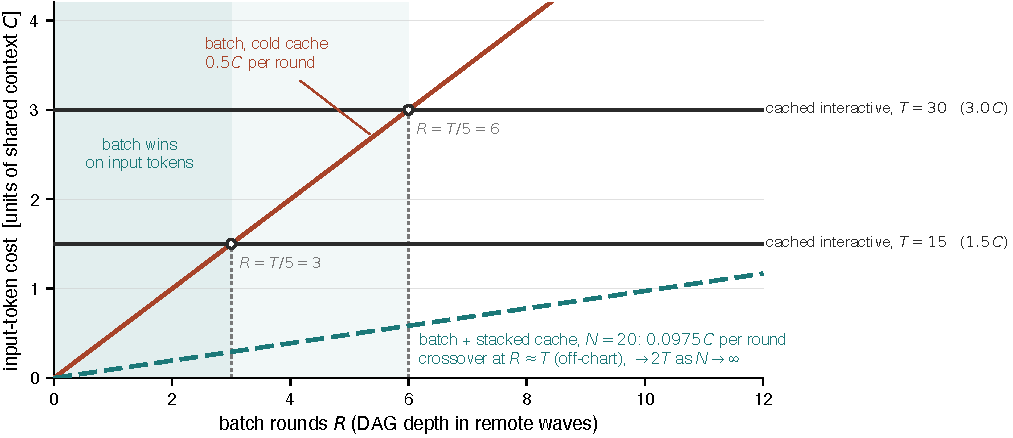
\includegraphics[width=\linewidth]{figures/economics.pdf}

\caption{\textbf{The economics condition.} Input-token cost of completing one task, in units of its shared context $C$, as a function of batch rounds $R$. A prompt-cached interactive agent pays $\approx 0.1\,C$ per turn (horizontal lines for $T{=}15$ and $T{=}30$ turns). Uncached batch pays $0.5\,C$ per round: it beats the cached baseline only left of the $R{=}T/5$ crossovers. With batch and cache discounts stacked across a wave of $N$ prefix-sharing items (dashed, $N{=}20$), the slope drops toward $0.05\,C$ and the crossover moves to $R \approx 2T$: width substitutes for depth-collapse. Output tokens (not shown) favor batch unconditionally at $\sim$50\%.}
\label{fig:economics}
\end{figure}

\section{The economics condition}
\label{sec:economics}

Let a task require shared context $C$ (repository slices, house rules, instructions). An interactive agent across $T$ turns re-reads that context every turn; with prompt caching, the input bill is approximately $0.1\,C\,T$ (cache writes and the uncached first turn add small constants). LazyCode front-loads the same context into each of $R$ batch rounds at the batch rate: $0.5\,C\,R$, assuming cold caches across waves. Batch wins on input iff
\[
0.5\,C\,R \;<\; 0.1\,C\,T \quad\Longleftrightarrow\quad \boxed{R < T/5}.
\]
A 30-turn interactive task compiled to 2--3 batch rounds costs $1.0$--$1.5\,C$ against the cached agent's $3.0\,C$; the same task compiled poorly, to 8 rounds, loses. Output tokens are never cacheable, so batch's 50\% discount on them is unconditional --- and agentic coding is output-heavy. The blended saving is therefore ``$\sim$50\% on output plus a conditional input win'': 30--70\% against a well-cached baseline, and the widely-quoted 60--85\% only against an uncached one. The design's own kill condition follows: if realized \texttt{rounds\_per\_node} degrades toward interactive depth, the input economics invert.

\subsection{Width changes the condition}
\label{sec:economics-width}

The derivation above assumes batch calls never hit caches. On current APIs that assumption is wrong in the favorable direction: batch and prompt-cache discounts \emph{stack}, and Anthropic explicitly recommends the 1-hour cache TTL for batch workloads. Within one wave, $N$ items sharing a hoisted prefix $C$ pay approximately $C \cdot 0.5 \cdot 2$ once (a 1-hour cache write at the batch rate, Anthropic's pricing) and $C \cdot 0.5 \cdot 0.1$ for the remaining $N{-}1$ reads --- \emph{when caching is worth requesting at all}. Because the cache write costs $2\times$, a rational renderer caches only when the wave is wide enough to amortize it, giving a piecewise per-item cost:
\[
\text{per-item input} \;\approx\; C\,R\cdot\min\!\Big(0.5,\; 0.05 + \tfrac{0.95}{N}\Big)
\quad\Longrightarrow\quad
\text{batch wins} \iff R\cdot\min\!\Big(0.5,\, 0.05+\tfrac{0.95}{N}\Big) < 0.1\,T .
\]
At $N{=}1$ the min selects the uncached branch and the condition is the original $R<T/5$; caching pays for $N \gtrsim 3$; at $N{=}20$, $R \lesssim T$; as $N \to \infty$, $R < 2T$. The arithmetic is Anthropic-specific (explicit cache-control with a $2\times$ 1-hour write); OpenAI's automatic positional caching has no write premium, making its optimistic form closer to $R(0.05+0.45/N)$ if the discounts stack there --- a provider-by-provider question the benchmark must settle empirically. Two further honesty notes: our own adapter does not yet request the 1-hour TTL (it sends the default 5-minute \texttt{ephemeral}; the upgrade is a one-line change, listed in \cref{sec:limitations}), and whether the 50\% batch discount applies to cache-read/write \emph{line items} is implied by provider ``stacking'' language but unverified by us. Two consequences. First, \emph{width is the real currency}: a coding agent must manufacture it by splitting one task along independence boundaries, but fleet workloads (evaluation sweeps, corpus processing) have width by construction --- the key fact behind \cref{sec:generalization}'s verdict. Second, cache hit rates are best-effort (providers cite 30--98\%); the honest statement is the sensitivity range, not a point estimate, and within-wave hit rate belongs in the benchmark suite as a first-class metric.

\subsection{The flex-tier confrontation}
\label{sec:flex}

OpenAI's flex tier delivers batch pricing on synchronous calls: one string, no architecture, minutes of extra latency instead of hours. Any defense of the batch-compilation architecture must therefore rest on what flex does \emph{not} provide: the 24-hour window that buys schedulable width (waves timed for cache stacking), the batch-exclusive server-side loop depth and 300k outputs, cross-run pooling, and --- on the self-hosted side --- the co-serving economics of the companion system (Tidal), where the batch tier monetizes idle capacity a flex-style tier would still consume at peak. For pure per-call discount on an interactive loop, flex dominates; this paper's architecture earns its complexity only where those additional properties are the point.

\section{Architecture}
\label{sec:architecture}

% FIGURE 2 SPEC (fig-pipeline.tex): the full pipeline block diagram, annotated. Horizontal flow:
% [User goal] -> [PLANNER realtime LLM: forced-tool Plan emission, 3-attempt schema retry]
% -> [LOGICAL PLAN: 8-operator typed DAG (validated: unique ids, resolvable deps, acyclic)]
% -> [OPTIMIZER: R1 LocalPushdown, R2 ContextPruning (shipped); R3-R10 designed (dimmed)]
% -> [PHYSICAL: layering, exec_class, (provider,model)] -> [WAVE LOOP: ready frontier ->
%    group by (provider,model) -> memo filter -> WAVE_FORMED -> submit -> poll -> process]
% -> [providers: Anthropic batch / OpenAI-compatible batch (Tidal!)] and side rails:
% [EVENT LOG (SQLite WAL): 23 event types, source of truth] under everything, with projections
% (jobs/nodes/waves) shown as derived; [WORKTREE: git apply --3way, applied_diffs ledger]
% [VERIFIER: user command] -> DONE / NEEDS_HUMAN. Annotate crash-safety windows W1/W2/W3
% between FORMED/SUBMITTED/COMPLETED. Use accent color for shipped, dimmed for designed-only.
\begin{figure}[!htbp]
\centering
% Figure 2 -- the LazyCode pipeline.
% accent = shipped code; dimmed/dashed = designed with plumbing, not reachable.
\resizebox{\linewidth}{!}{%
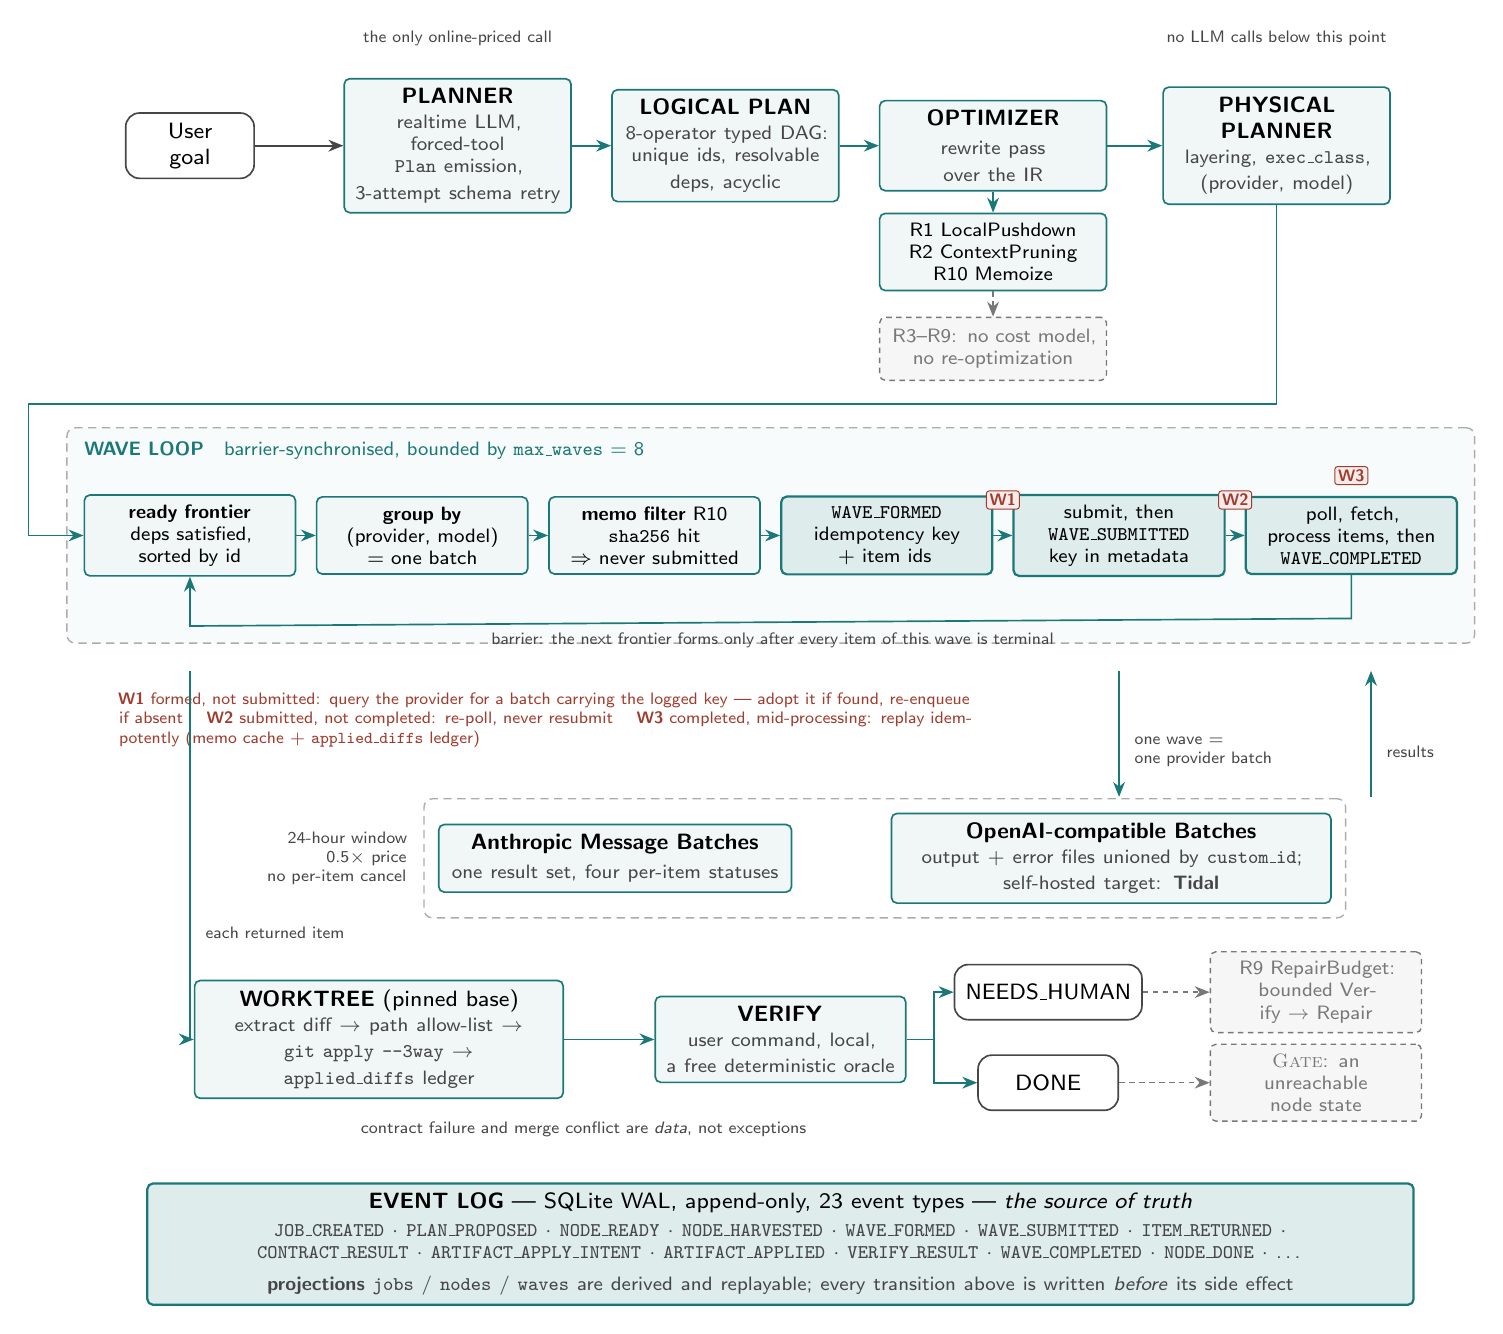
\begin{tikzpicture}[x=1cm,y=1cm]

\tikzset{
  wtag/.append style={fill=danger!10, rounded corners=1pt, draw=danger, line width=0.35pt,
                      font=\sffamily\bfseries\fontsize{6}{7}\selectfont},
}

% =============== ROW A: plan time, priced online ===========================
\node[term, text width=1.35cm] (goal) at (0.9,0) {User\\goal};
\node[box, text width=2.6cm]  (plan) at (4.3,0)
  {\textbf{PLANNER}\\[1pt]\lbltext{realtime LLM, forced-tool\\ \texttt{Plan} emission,\\
   3-attempt schema retry}};
\node[box, text width=2.6cm] (lp) at (7.7,0)
  {\textbf{LOGICAL PLAN}\\[1pt]\lbltext{8-operator typed DAG:\\ unique ids, resolvable\\
   deps, acyclic}};
\node[box, text width=2.6cm] (opt) at (11.1,0)
  {\textbf{OPTIMIZER}\\[1pt]\lbltext{rewrite pass over the IR}};
\node[box, text width=2.6cm] (phys) at (14.7,0)
  {\textbf{PHYSICAL PLANNER}\\[1pt]\lbltext{layering, \texttt{exec\_class},\\ (provider, model)}};

\node[boxs, text width=2.6cm] (optS) at (11.1,-1.35)
  {R1 LocalPushdown\\ R2 ContextPruning\\ R10 Memoize};
\node[dboxs, text width=2.6cm] (optD) at (11.1,-2.58)
  {R3--R9: no cost model,\\ no re-optimization};

\draw[arg] (goal) -- (plan);
\draw[ar]  (plan) -- (lp);
\draw[ar]  (lp)   -- (opt);
\draw[ar]  (opt)  -- (phys);
\draw[ar]  (opt.south) -- (optS.north);
\draw[dar] (optS.south) -- (optD.north);

\node[lbls, anchor=south] at (4.3,1.22) {the only online-priced call};
\node[lbls, anchor=south] at (14.7,1.22) {no LLM calls below this point};

% =============== ROW B: the wave loop ======================================
\def\wy{-4.95}
\node[boxs, text width=2.4cm] (fr)   at (0.9,\wy)
  {\textbf{ready frontier}\\ deps satisfied,\\ sorted by id};
\node[boxs, text width=2.4cm] (grp)  at (3.85,\wy)
  {\textbf{group by}\\ (provider, model)\\ $=$ one batch};
\node[boxs, text width=2.4cm] (memo) at (6.8,\wy)
  {\textbf{memo filter} R10\\ \texttt{sha256} hit\\ $\Rightarrow$ never submitted};
\node[boxf, text width=2.4cm, font=\sffamily\scriptsize] (formed) at (9.75,\wy)
  {\texttt{WAVE\_FORMED}\\ idempotency key\\ $+$ item ids};
\node[boxf, text width=2.4cm, font=\sffamily\scriptsize] (subm) at (12.7,\wy)
  {submit, then\\ \texttt{WAVE\_SUBMITTED}\\ key in metadata};
\node[boxf, text width=2.4cm, font=\sffamily\scriptsize] (poll) at (15.65,\wy)
  {poll, fetch,\\ process items, then\\ \texttt{WAVE\_COMPLETED}};

\draw[ar] (fr) -- (grp);
\draw[ar] (grp) -- (memo);
\draw[ar] (memo) -- (formed);
\draw[ar] (formed) -- (subm);
\draw[ar] (subm) -- (poll);

\node[wtag] at (11.225,\wy+0.45) {W1};
\node[wtag] at (14.175,\wy+0.45) {W2};
\node[wtag] at (15.65,\wy+0.76) {W3};

\begin{scope}[on background layer]
  \node[group, fill=accent!3, fit=(fr)(poll), inner xsep=6pt, inner ysep=24pt] (waveloop) {};
\end{scope}
\node[banner, anchor=north west] at ([xshift=3pt,yshift=-2pt]waveloop.north west)
  {WAVE LOOP \; \normalfont\sffamily\scriptsize
   barrier-synchronised, bounded by \texttt{max\_waves} $=$ 8};

% barrier feedback edge, inside the container's bottom padding
\draw[ar] (poll.south) -- ++(0,-0.55) -- (0.9,\wy-1.15) -- (fr.south);
\node[lbls, anchor=north] at (8.3,\wy-1.19)
  {barrier: the next frontier forms only after every item of this wave is terminal};

\draw[ar] (phys.south) -- (14.7,-3.28) -- (-1.15,-3.28) -- (-1.15,\wy) -- (fr.west);

% crash windows, explained below the loop
\node[lbls, text=danger, anchor=north, align=left, text width=10.8cm] at (5.4,\wy-1.95)
  {\textbf{W1} formed, not submitted: query the provider for a batch carrying the logged key
   \textemdash{} adopt it if found, re-enqueue if absent \quad
   \textbf{W2} submitted, not completed: re-poll, never resubmit \quad
   \textbf{W3} completed, mid-processing: replay idempotently (memo cache $+$
   \texttt{applied\_diffs} ledger)};

% =============== ROW B2: providers =========================================
\def\py{-9.05}
\node[box, text width=4.2cm] (anth) at (6.3,\py)
  {\textbf{Anthropic Message Batches}\\[1pt]\lbltext{one result set, four per-item statuses}};
\node[box, text width=5.3cm] (oai) at (12.6,\py)
  {\textbf{OpenAI-compatible Batches}\\[1pt]\lbltext{output $+$ error files unioned by
   \texttt{custom\_id};\\ self-hosted target: \textbf{Tidal}}};
\node[lbls, anchor=east, align=right, text width=2.6cm] at (3.7,\py)
  {24-hour window\\ 0.5$\times$ price\\ no per-item cancel};
\begin{scope}[on background layer]
  \node[group, fit=(anth)(oai), inner sep=5pt] (provs) {};
\end{scope}

\draw[ar] (12.7,\wy-1.72) -- (12.7,\py+0.78);
\node[lbls, anchor=west, align=left, text width=2.5cm] at (12.85,\py+1.35) {one wave $=$\\ one provider batch};
\draw[ar] (15.9,\py+0.78) -- (15.9,\wy-1.72);
\node[lbls, anchor=west, align=left] at (16.05,\py+1.35) {results};

% =============== ROW C: apply / verify =====================================
\def\cy{-11.35}
\node[box, text width=4.4cm] (wt) at (3.3,\cy)
  {\textbf{WORKTREE} (pinned base)\\[1pt]\lbltext{extract diff $\to$ path allow-list $\to$\\
   \texttt{git apply -{}-3way} $\to$ \texttt{applied\_diffs} ledger}};
\node[box, text width=2.9cm] (ver) at (8.4,\cy)
  {\textbf{VERIFY}\\[1pt]\lbltext{user command, local,\\ a free deterministic oracle}};
\node[term, text width=1.5cm] (done) at (11.8,\cy-0.55) {DONE};
\node[term, text width=2.1cm] (nh)   at (11.8,\cy+0.6) {NEEDS\_HUMAN};
\node[dboxs, text width=2.4cm] (rep) at (15.2,\cy+0.6)
  {R9 RepairBudget:\\ bounded Verify $\to$ Repair};
\node[dboxs, text width=2.4cm] (gate) at (15.2,\cy-0.55)
  {\textsc{Gate}: an unreachable\\ node state};

\draw[ar] (0.9,\wy-1.72) -- (0.9,\cy) -- (wt.west);
\node[lbls, anchor=west, align=left, text width=2.2cm] at (1.05,\cy+1.35)
  {each returned item};
\draw[ar] (wt) -- (ver);
\draw[ar] (ver.east) -- ++(0.35,0) |- (done.west);
\draw[ar] (ver.east) -- ++(0.35,0) |- (nh.west);
\draw[dar] (nh) -- (rep);
\draw[dar] (done) -- (gate);
\node[lbls, anchor=north, align=center, text width=6.5cm] at (5.9,\cy-1.0)
  {contract failure and merge conflict are \emph{data}, not exceptions};

% =============== BOTTOM RAIL: event log ====================================
\def\ey{-13.95}
\node[boxf, text width=15.8cm, minimum height=11mm] (log) at (8.4,\ey)
  {\textbf{EVENT LOG} \textemdash{} SQLite WAL, append-only, 23 event types
   \textemdash{} \emph{the source of truth}\\[2pt]
   \lbltext{\texttt{JOB\_CREATED} $\cdot$ \texttt{PLAN\_PROPOSED} $\cdot$ \texttt{NODE\_READY}
   $\cdot$ \texttt{NODE\_HARVESTED} $\cdot$ \texttt{WAVE\_FORMED} $\cdot$
   \texttt{WAVE\_SUBMITTED} $\cdot$ \texttt{ITEM\_RETURNED} $\cdot$ \texttt{CONTRACT\_RESULT}
   $\cdot$ \texttt{ARTIFACT\_APPLY\_INTENT} $\cdot$ \texttt{ARTIFACT\_APPLIED} $\cdot$
   \texttt{VERIFY\_RESULT} $\cdot$ \texttt{WAVE\_COMPLETED} $\cdot$ \texttt{NODE\_DONE}
   $\cdot$ \dots\\[2pt]
   \textbf{projections} \texttt{jobs} / \texttt{nodes} / \texttt{waves} are derived and
   replayable; every transition above is written \emph{before} its side effect}};

\end{tikzpicture}}

\caption{\textbf{The LazyCode pipeline.} Solid/accent components are shipped code; dimmed components are designed with plumbing but not yet live (\cref{sec:implementation}). The event log is the source of truth; \texttt{jobs}/\texttt{nodes}/\texttt{waves} tables are replayable projections. W1--W3 mark the three crash-safety windows of \cref{sec:crash}.}
\label{fig:pipeline}
\end{figure}

\subsection{The logical plan: an algebra of engineering work}

Eight typed operators form the planning vocabulary: \textsc{Explore}, \textsc{Decompose}, \textsc{Generate}, \textsc{Edit}, \textsc{Verify}, \textsc{Judge}, \textsc{Reduce}, \textsc{Gate}. Only \textsc{Generate} and \textsc{Edit} carry a \texttt{context\_spec} (what to harvest) and an \texttt{output\_contract} (what shape must come back) --- they are the operators that spend money and mutate the tree. The plan is a Pydantic-validated DAG: unique ids, resolvable dependencies (including \texttt{"node.*"} fan-out patterns), acyclicity by iterative DFS. Critically, the planner cannot drift from this schema, because the planning prompt's tool definition \emph{is} \texttt{Plan.model\_json\_schema()} and the algebra documentation shown to the model is generated from the model fields themselves; a validation error is fed back verbatim for up to three repair attempts.

The DAG-shape thesis is executable prompt text, quoted in full because it is the paper's mechanism in one sentence:
\begin{quote}\itshape
``Structure the work as a shallow, WIDE DAG (few dependency layers, much fan-out) because wall-clock is proportional to DAG depth: split independent work (per-file, per-module) into sibling nodes at the same layer instead of chaining it.''
\end{quote}

\subsection{The optimizer: rules with database analogues}

\Cref{tab:rules} lists the ten rewrite rules with their database lineage. Two rewrites ship today, plus R10 --- an execution-layer memoization rather than a plan rewrite; the table's Status column is load-bearing (\cref{sec:implementation}).

\begin{table}[!htbp]
\centering\small
\caption{Optimizer rules, their database analogues, and implementation status. ``Plumbed'' = data model and call paths exist; the decision logic does not.}
\label{tab:rules}
\begin{tabular}{@{}lllp{5.6cm}@{}}
\toprule
Rule & DB analogue & Status & Semantics \\
\midrule
R1 LocalPushdown & predicate pushdown & \textbf{shipped}$^{*}$ & planner-flagged \textsc{Explore} executes locally, free, no LLM round ($^{*}$the flag is trusted, not analyzed, and local execution today yields a scope artifact rather than tool output --- \cref{sec:implementation}) \\
R2 ContextPruning & projection pruning & \textbf{shipped} & nodes touching $\le$2 literal files drop the repo map from their context \\
R3 FanoutWidening & join reordering & prompt-level & split coarse nodes along independence boundaries; today width comes from the planner prompt, not a rewrite \\
R4 PrefixFactoring & common subexpr.\ elim. & partial & shared context hoisted to a cache-hinted prefix block; per-call today, not per-wave \\
R5 ModelTiering & access-path selection & designed & cheapest model whose predicted verify-pass rate clears threshold; escalate on failure \\
R6 Vectorize & batched row processing & plumbed & pack $k$ homogeneous tasks into one call; \texttt{call\_items} maps 1 call to $k$ nodes ($k{=}1$ today) \\
R7 Speculate & branch prediction & designed & submit enumerable continuations as siblings --- restricted to \emph{remote}-decider branches after review showed the local-decider case saves zero waves \\
R8 HedgeInsertion & hedged reads & designed & stall detection + realtime duplicate for critical-path items \\
R9 RepairBudget & --- & designed & bounded Verify$\to$Repair loops, then \textsc{needs\_human} \\
R10 Memoize & materialized views & \textbf{shipped} & \texttt{sha256(model, prompt, mode, sample\_idx)} keys an exact-reuse cache; identical calls never re-bill \\
\bottomrule
\end{tabular}
\end{table}

\subsection{Wave formation and the barrier ruling}

The scheduler runs a bounded loop over the \emph{ready frontier}: nodes whose dependencies are all successful, sorted by id for deterministic apply order. Remote frontier nodes group by (provider, model); each group becomes exactly one provider batch --- a \emph{wave}. Waves are barriers: the whole frontier submits, the orchestrator polls to completion, results are processed, and only then does the next frontier form. The design review's most contested ruling chose barriers over rolling flushes, for two reasons that compound: the cost model stays literal (wall-clock $\approx$ depth $\times$ wave latency) and the acceptance test stays countable. Rolling execution is deferred, not rejected.

Wave identity is \emph{content-addressed}: the idempotency key is a hash of the rendered items plus a flush ordinal recovered by scanning the durable log --- not an in-memory counter --- so a crashed-and-resumed orchestrator derives the same key and can adopt its own orphaned submission.

% FIGURE 3 SPEC (fig-plan-example.tex): before/after plan rewrite, two small DAGs side by side.
% LEFT "as planned": Explore(find modules) -> Decompose -> 3x Generate(tests for m1,m2,m3) -> Verify -> Reduce
% shown as a chain-heavy DAG with repo_map=true on all Generate nodes.
% RIGHT "as optimized/lowered": Explore becomes LOCAL (R1, accent border, "$0, 0 rounds");
% Generate nodes at same layer (wave 1) each annotated "repo_map dropped (R2)" where files<=2;
% wave boundaries drawn as horizontal dashed bands labeled wave-0 (local, free), wave-1 (batch),
% wave-2 (verify local). Annotate: "depth 2 remote rounds; width 3".
\begin{figure}[!htbp]
\centering
% Figure 3 -- a plan, compiled: logical DAG (left) vs. rewritten + lowered (right).
\resizebox{\linewidth}{!}{%
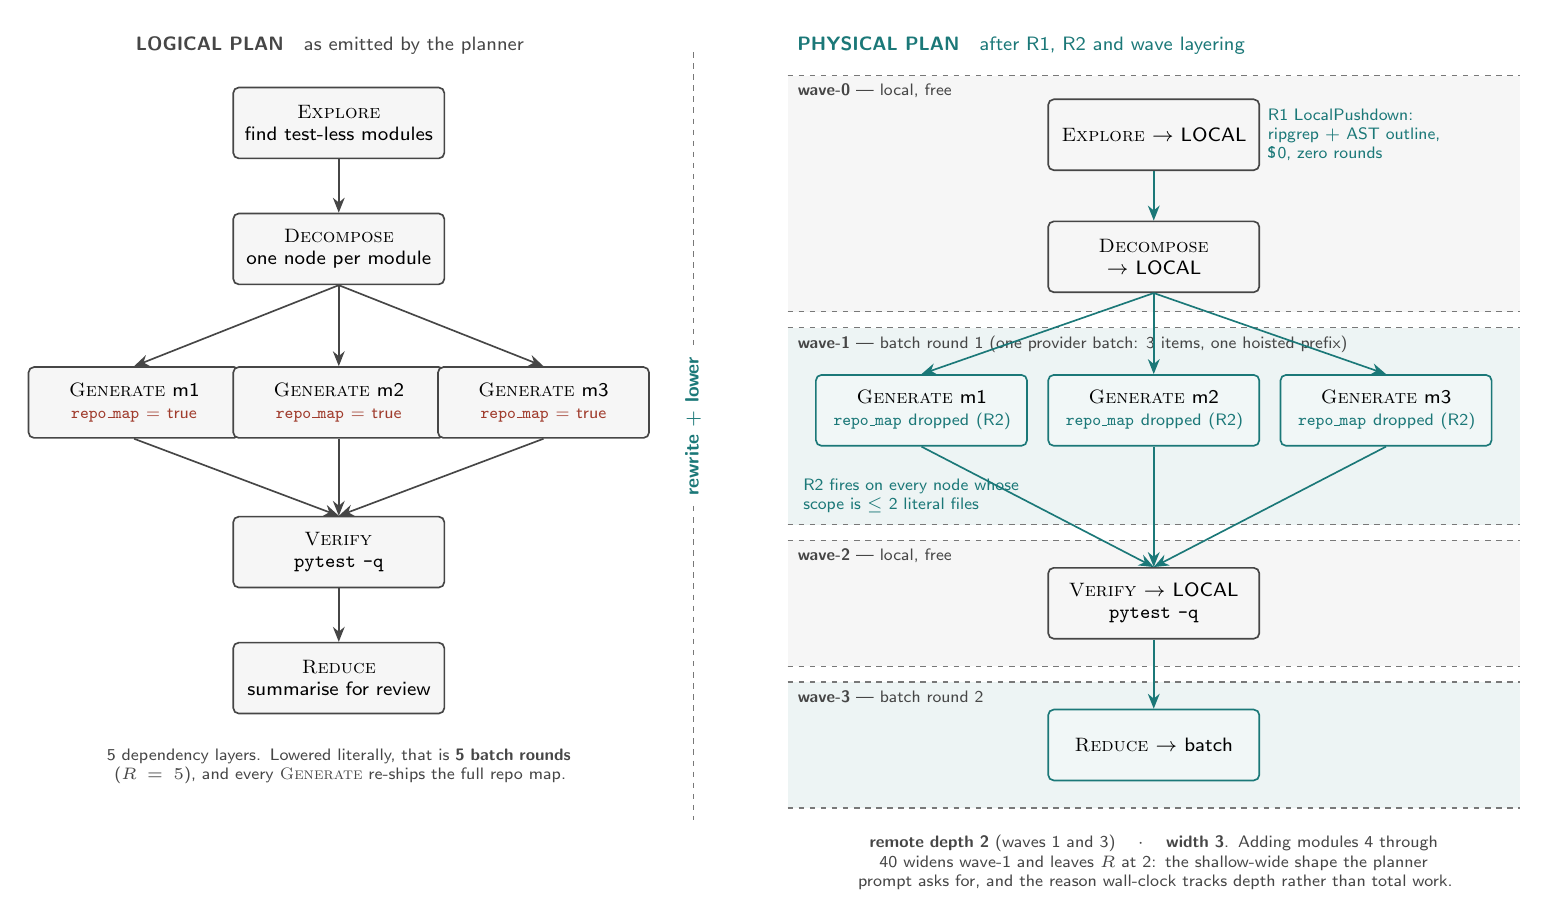
\begin{tikzpicture}[x=1cm,y=1cm]

\tikzset{
  opn/.style={box, text width=2.4cm, minimum height=9mm, font=\sffamily\scriptsize},
  opl/.style={opn, draw=inkgray, fill=inkgray!5},
  note/.style={lbls, anchor=north, text width=2.5cm},
}

% ============================ LEFT: as planned =============================
\node[banner, anchor=south west, text=inkgray] at (-0.1,1.3)
  {LOGICAL PLAN \; \normalfont\sffamily\scriptsize as emitted by the planner};

\node[opl] (lex)  at (2.6,0.55)  {\textsc{Explore}\\ find test-less modules};
\node[opl] (ldec) at (2.6,-1.05) {\textsc{Decompose}\\ one node per module};
\node[opl] (lg1)  at (0.0,-3.0)
  {\textsc{Generate} m1\\ \lbltiny{\textcolor{danger}{\texttt{repo\_map} = true}}};
\node[opl] (lg2)  at (2.6,-3.0)
  {\textsc{Generate} m2\\ \lbltiny{\textcolor{danger}{\texttt{repo\_map} = true}}};
\node[opl] (lg3)  at (5.2,-3.0)
  {\textsc{Generate} m3\\ \lbltiny{\textcolor{danger}{\texttt{repo\_map} = true}}};
\node[opl] (lver) at (2.6,-4.9) {\textsc{Verify}\\ \texttt{pytest -q}};
\node[opl] (lred) at (2.6,-6.5) {\textsc{Reduce}\\ summarise for review};

\draw[arg] (lex) -- (ldec);
\foreach \n in {lg1,lg2,lg3} { \draw[arg] (ldec.south) -- (\n.north); }
\foreach \n in {lg1,lg2,lg3} { \draw[arg] (\n.south) -- (lver.north); }
\draw[arg] (lver) -- (lred);

\node[lbls, anchor=north, text width=6.4cm] at (2.6,-7.35)
  {5 dependency layers. Lowered literally, that is \textbf{5 batch rounds}
   ($R = 5$), and every \textsc{Generate} re-ships the full repo map.};

% separator
\draw[dimmed, dash pattern=on 2pt off 2pt] (7.1,1.45) -- (7.1,-8.3);
\node[lbl, text=accent, fill=white, inner sep=3pt] at (7.1,-3.3)
  {\rotatebox{90}{\textbf{rewrite $+$ lower}}};

% ====================== RIGHT: rewritten and lowered =======================
\def\bandL{8.3}\def\bandR{17.6}
\newcommand{\band}[4]{%
  \fill[#4] (\bandL,#1) rectangle (\bandR,#2);
  \draw[dimmed, dash pattern=on 2pt off 2pt] (\bandL,#1) -- (\bandR,#1);
  \draw[dimmed, dash pattern=on 2pt off 2pt] (\bandL,#2) -- (\bandR,#2);
  \node[lbls, anchor=north west, align=left] at (\bandL+0.08,#2-0.06) {#3};}

\node[banner, anchor=south west] at (\bandL,1.3)
  {PHYSICAL PLAN \; \normalfont\sffamily\scriptsize after R1, R2 and wave layering};

\band{-1.85}{1.15}{\textbf{wave-0} \textemdash{} local, free}{inkgray!5}
\band{-4.55}{-2.05}{\textbf{wave-1} \textemdash{} batch round 1 (one provider batch:
  3 items, one hoisted prefix)}{accent!8}
\band{-6.35}{-4.75}{\textbf{wave-2} \textemdash{} local, free}{inkgray!5}
\band{-8.15}{-6.55}{\textbf{wave-3} \textemdash{} batch round 2}{accent!8}

\node[opl] (rex)  at (12.95,0.4)  {\textsc{Explore} $\to$ LOCAL};
\node[opl] (rdec) at (12.95,-1.15) {\textsc{Decompose} $\to$ LOCAL};
\node[lbls, anchor=west, align=left, text width=3.3cm, text=accent] at (14.35,0.4)
  {R1 LocalPushdown:\\ ripgrep $+$ AST outline,\\ \$0, zero rounds};

\node[opn] (rg1) at (10.0,-3.10)
  {\textsc{Generate} m1\\ \lbltiny{\textcolor{accent}{\texttt{repo\_map} dropped (R2)}}};
\node[opn] (rg2) at (12.95,-3.10)
  {\textsc{Generate} m2\\ \lbltiny{\textcolor{accent}{\texttt{repo\_map} dropped (R2)}}};
\node[opn] (rg3) at (15.9,-3.10)
  {\textsc{Generate} m3\\ \lbltiny{\textcolor{accent}{\texttt{repo\_map} dropped (R2)}}};
\node[lbls, anchor=north west, align=left, text=accent, text width=4.4cm] at (8.45,-3.92)
  {R2 fires on every node whose\\ scope is $\le$ 2 literal files};

\node[opl] (rver) at (12.95,-5.55) {\textsc{Verify} $\to$ LOCAL\\ \texttt{pytest -q}};
\node[opn] (rred) at (12.95,-7.35) {\textsc{Reduce} $\to$ batch};

\draw[ar] (rex) -- (rdec);
\foreach \n in {rg1,rg2,rg3} { \draw[ar] (rdec.south) -- (\n.north); }
\foreach \n in {rg1,rg2,rg3} { \draw[ar] (\n.south) -- (rver.north); }
\draw[ar] (rver) -- (rred);

\node[lbls, anchor=north, text width=8.8cm, align=center] at (12.95,-8.45)
  {\textbf{remote depth 2} (waves 1 and 3) $\;\cdot\;$ \textbf{width 3}.
   Adding modules 4 through 40 widens wave-1 and leaves $R$ at 2: the shallow-wide
   shape the planner prompt asks for, and the reason wall-clock tracks depth rather
   than total work.};

\end{tikzpicture}}

\caption{\textbf{A plan, compiled.} Left: the planner's logical DAG for ``add tests for three modules.'' Right: after rewriting and lowering --- the \textsc{Explore} is pushed to free local execution (R1), trivially-scoped \textsc{Generate} nodes shed their repo map (R2), and layering yields two remote rounds regardless of module count: depth stays constant while width scales.}
\label{fig:plan-example}
\end{figure}

\subsection{Crash safety: three windows, three recoveries}
\label{sec:crash}

A batch submission is a paid, remote, irrevocable side effect, and the system treats it with WAL discipline. \texttt{WAVE\_FORMED} --- carrying the idempotency key and item ids --- is durably logged \emph{before} any provider call; \texttt{WAVE\_SUBMITTED} after; \texttt{WAVE\_COMPLETED} only after every returned item is fully processed. Each window has a distinct recovery: (W1) formed-not-submitted resolves by querying the provider for a batch bearing the logged key --- found means adopt, absent means re-enqueue; (W2) submitted-not-completed re-polls and never resubmits; (W3) completed-mid-processing replays idempotently, because item results route through the memo cache and diff application checks a content-hash ledger before touching the worktree. Independent belts and braces: provider-side metadata, log-derived keys, the \texttt{applied\_diffs} ledger, and a \texttt{UNIQUE(memo\_key)} constraint on the spend cache. This is the strongest-implemented subsystem (\cref{sec:implementation}), and deliberately so: in an architecture whose entire premise is unattended execution, recovery is the product.

\section{From interactive intent to self-sufficient calls}
\label{sec:selfsufficiency}

% FIGURE 5 SPEC (fig-callanatomy.tex): anatomy of one rendered batch call, a tall annotated box:
% [system: execution role ("You are a lazycode batch executor... cannot ask questions...
%   record under 'Assumptions:'")] / [prefix block: repo map (cache_hint=true) - annotate "R4 hoist,
%   byte budget 8KB"] / [prefix: house rules (16 candidate files, 20KB budget)] /
% [user msg: instruction + "### File:" blocks (60KB/file, 400KB total, overflow -> omitted list)
%   + contract directive ("SINGLE unified diff... Only touch files matching: <globs>...
%   Assumptions AFTER the diff")] -> arrows out: [memo_key = sha256(model, prompt, mode, idx)]
% and return path: [extract_diff -> path allowlist check -> git apply --3way -> ledger]
% plus [Assumptions: ...] flowing to [morning report]. Annotate byte budgets on each block.
\begin{figure}[!htbp]
\centering
% Figure 5 -- anatomy of one rendered, self-sufficient batch call.
% Prompt strings quoted verbatim from lazycode/scheduler/render.py;
% byte budgets from lazycode/harvest/harvester.py.
\resizebox{\linewidth}{!}{%
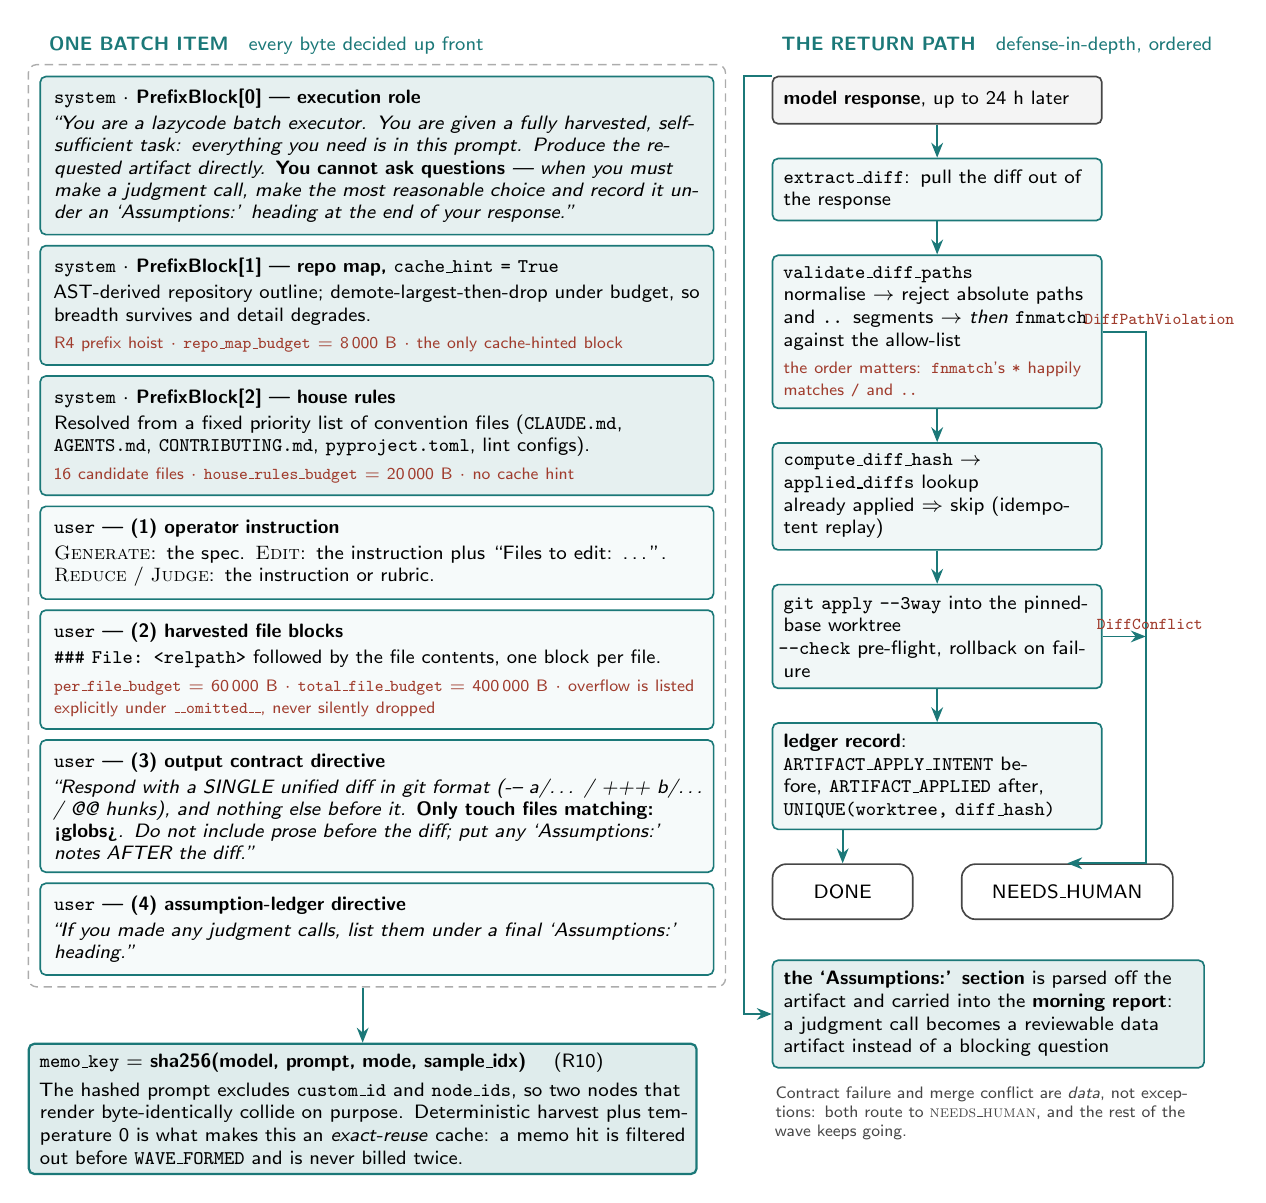
\begin{tikzpicture}[x=1cm,y=1cm]

\tikzset{
  blk/.style={box, text width=8.2cm, align=left, font=\sffamily\scriptsize,
              inner xsep=5pt, inner ysep=4.5pt},
  sysblk/.style={blk, fill=accent!11},
  usrblk/.style={blk, fill=accent!4},
  rblk/.style={boxs, text width=3.9cm, align=left, minimum height=6mm,
               inner xsep=4pt, inner ysep=4pt,
               font=\sffamily\fontsize{6.8}{8.2}\selectfont},
}

\newcommand{\hdr}[1]{\textbf{#1}\\[1.5pt]}
\newcommand{\qtext}[1]{{\sffamily\fontsize{6.6}{8}\selectfont\itshape #1}}
\newcommand{\budget}[1]{{\sffamily\fontsize{6.2}{7.4}\selectfont\color{danger}#1}}

% ======================= LEFT COLUMN: the rendered call ====================
\node[banner, anchor=south west] at (0,4.6)
  {ONE BATCH ITEM \; \normalfont\sffamily\scriptsize every byte decided up front};

\node[sysblk, anchor=north west] (sys) at (0,4.45)
  {\hdr{\texttt{system} $\cdot$ PrefixBlock[0] \textemdash{} execution role}
   \qtext{``You are a lazycode batch executor. You are given a fully harvested,
   self-sufficient task: everything you need is in this prompt. Produce the
   requested artifact directly. \textbf{You cannot ask questions} \textemdash{} when you
   must make a judgment call, make the most reasonable choice and record it
   under an `Assumptions:' heading at the end of your response.''}};

\node[sysblk, below=1.2mm of sys.south west, anchor=north west] (rmap)
  {\hdr{\texttt{system} $\cdot$ PrefixBlock[1] \textemdash{} repo map, \texttt{cache\_hint = True}}
   AST-derived repository outline; demote-largest-then-drop under budget, so breadth
   survives and detail degrades.\\[2pt]
   \budget{R4 prefix hoist $\cdot$ \texttt{repo\_map\_budget} $=$ 8\,000 B $\cdot$
   the only cache-hinted block}};

\node[sysblk, below=1.2mm of rmap.south west, anchor=north west] (rules)
  {\hdr{\texttt{system} $\cdot$ PrefixBlock[2] \textemdash{} house rules}
   Resolved from a fixed priority list of convention files (\texttt{CLAUDE.md},
   \texttt{AGENTS.md}, \texttt{CONTRIBUTING.md}, \texttt{pyproject.toml}, lint configs).\\[2pt]
   \budget{16 candidate files $\cdot$ \texttt{house\_rules\_budget} $=$ 20\,000 B
   $\cdot$ no cache hint}};

\node[usrblk, below=1.2mm of rules.south west, anchor=north west] (instr)
  {\hdr{\texttt{user} \textemdash{} (1) operator instruction}
   \textsc{Generate}: the spec. \textsc{Edit}: the instruction plus ``Files to edit:
   \dots''. \textsc{Reduce} / \textsc{Judge}: the instruction or rubric.};

\node[usrblk, below=1.2mm of instr.south west, anchor=north west] (files)
  {\hdr{\texttt{user} \textemdash{} (2) harvested file blocks}
   \texttt{\#\#\# File: <relpath>} followed by the file contents, one block per file.\\[2pt]
   \budget{\texttt{per\_file\_budget} $=$ 60\,000 B $\cdot$ \texttt{total\_file\_budget}
   $=$ 400\,000 B $\cdot$ overflow is listed explicitly under \texttt{\_\_omitted\_\_},
   never silently dropped}};

\node[usrblk, below=1.2mm of files.south west, anchor=north west] (contract)
  {\hdr{\texttt{user} \textemdash{} (3) output contract directive}
   \qtext{``Respond with a SINGLE unified diff in git format
   (-{}-- a/\dots\ / +++ b/\dots\ / @@ hunks), and nothing else before it.
   \textbf{Only touch files matching: <globs>}. Do not include prose before the diff;
   put any `Assumptions:' notes AFTER the diff.''}};

\node[usrblk, below=1.2mm of contract.south west, anchor=north west] (assume)
  {\hdr{\texttt{user} \textemdash{} (4) assumption-ledger directive}
   \qtext{``If you made any judgment calls, list them under a final
   `Assumptions:' heading.''}};

\begin{scope}[on background layer]
  \node[group, fit=(sys)(assume), inner xsep=4pt, inner ysep=4pt] (call) {};
\end{scope}

% ---- memo key -------------------------------------------------------------
\node[boxf, text width=8.2cm, below=7mm of call.south west, anchor=north west, align=left,
      font=\sffamily\fontsize{6.8}{8.2}\selectfont] (memo)
  {\textbf{\texttt{memo\_key} $=$ sha256(model, prompt, mode, sample\_idx)} \quad (R10)\\[2pt]
   The hashed prompt excludes \texttt{custom\_id} and \texttt{node\_ids}, so two nodes that
   render byte-identically collide on purpose. Deterministic harvest plus temperature 0 is
   what makes this an \emph{exact-reuse} cache: a memo hit is filtered out before
   \texttt{WAVE\_FORMED} and is never billed twice.};
\draw[ar] (call.south -| memo.north) -- (memo.north);

% ======================= RIGHT COLUMN: the return path =====================
\def\rx{9.3}
\node[banner, anchor=south west] at (\rx,4.6)
  {THE RETURN PATH \; \normalfont\sffamily\scriptsize defense-in-depth, ordered};

\node[rblk, anchor=north west, fill=inkgray!6, draw=inkgray] (resp) at (\rx,4.45)
  {\textbf{model response}, up to 24 h later};
\node[rblk, below=4.2mm of resp.south west, anchor=north west] (ext)
  {\textbf{\texttt{extract\_diff}}: pull the diff out of the response};
\node[rblk, below=4.2mm of ext.south west, anchor=north west] (val)
  {\textbf{\texttt{validate\_diff\_paths}}\\
   normalise $\to$ reject absolute paths and \texttt{..} segments $\to$
   \emph{then} \texttt{fnmatch} against the allow-list\\[1.5pt]
   \budget{the order matters: \texttt{fnmatch}'s \texttt{*} happily matches
   \texttt{/} and \texttt{..}}};
\node[rblk, below=4.2mm of val.south west, anchor=north west] (hash)
  {\textbf{\texttt{compute\_diff\_hash}} $\to$ \texttt{applied\_diffs} lookup\\
   already applied $\Rightarrow$ skip (idempotent replay)};
\node[rblk, below=4.2mm of hash.south west, anchor=north west] (apply)
  {\textbf{\texttt{git apply -{}-3way}} into the pinned-base worktree\\
   \texttt{-{}-check} pre-flight, rollback on failure};
\node[rblk, below=4.2mm of apply.south west, anchor=north west] (ledger)
  {\textbf{ledger record}: \texttt{ARTIFACT\_APPLY\_INTENT} before,
   \texttt{ARTIFACT\_APPLIED} after, \texttt{UNIQUE(worktree, diff\_hash)}};

\node[term, below=4.2mm of ledger.south west, anchor=north west, text width=1.5cm,
      font=\sffamily\scriptsize] (done) {DONE};
\node[term, right=6mm of done, text width=2.4cm, font=\sffamily\scriptsize] (nh)
  {NEEDS\_HUMAN};

\draw[ar] (resp) -- (ext);
\draw[ar] (ext) -- (val);
\draw[ar] (val) -- (hash);
\draw[ar] (hash) -- (apply);
\draw[ar] (apply) -- (ledger);
\draw[ar] (ledger.south -| done.north) -- (done.north);

\coordinate (fx) at (14.05,0);
\draw[ar] (val.east) -- (val.east -| fx) -- (fx |- nh.north) -- (nh.north);
\node[lbls, anchor=south, text=danger] at ($(val.east)+(0.72,0.04)$) {\texttt{DiffPathViolation}};
\draw[ar] (apply.east) -- (apply.east -| fx);
\node[lbls, anchor=south, text=danger] at ($(apply.east)+(0.6,0.04)$) {\texttt{DiffConflict}};

\node[rblk, below=5mm of done.south west, anchor=north west, fill=accent!12,
      text width=5.2cm] (asm)
  {\textbf{the `Assumptions:' section} is parsed off the artifact and carried into the
   \textbf{morning report}: a judgment call becomes a reviewable data artifact instead of
   a blocking question};
\draw[ar] (resp.north west) -- ++(-0.35,0) |- (asm.west);
\node[lbls, anchor=north west, align=left, text width=5.2cm]
  at ($(asm.south west)+(0,-0.18)$)
  {Contract failure and merge conflict are \emph{data}, not exceptions: both route to
   \textsc{needs\_human}, and the rest of the wave keeps going.};

\end{tikzpicture}}

\caption{\textbf{Anatomy of a self-sufficient call.} Every byte the model will see is decided before submission, under explicit budgets; the output contract constrains the return shape; judgment calls come back as a structured \emph{Assumptions} section feeding the morning report rather than blocking execution.}
\label{fig:callanatomy}
\end{figure}

Three mechanisms convert interactive intent into deferred execution.

\paragraph{Front-loaded harvest under byte budgets.} Context is gathered \emph{before} submission, deterministically: an AST-derived repository outline (demote-largest-then-drop under an 8\,KB budget --- breadth survives, detail degrades), the referenced files (60\,KB each, 400\,KB total, overflow explicitly listed as omitted), and house rules resolved from a fixed priority list of convention files. Determinism matters twice over: identical repo state yields byte-identical context, which is what makes the memo key (R10) an exact-reuse cache rather than a heuristic one.

\paragraph{Contracts on the way back.} A \textsc{Generate}/\textsc{Edit} node declares its output contract --- today, a unified diff confined to a glob allow-list. Validation is defense-in-depth ordered: path normalization rejects absolute paths and traversal \emph{before} glob matching (because \texttt{fnmatch}'s \texttt{*} happily matches \texttt{/} and \texttt{..}), then a three-way \texttt{git apply} against a pinned-base worktree, with rollback on conflict and a content-hash ledger making application idempotent. Contract failure and merge conflict both route to \textsc{needs\_human} --- failure is data, not an exception.

\paragraph{The assumption ledger.} The prompt contract states it plainly: \emph{``You cannot ask questions --- when you must make a judgment call, make the most reasonable choice and record it under an `Assumptions:' heading.''} The planner records its own scope-level judgment calls in the plan; executors append theirs after each artifact. What would be a blocking clarification in an interactive loop becomes a reviewable data artifact in the morning report. This is the interaction-model transplant in miniature --- and, we will argue, the single most portable idea in the system (\cref{sec:generalization}).

\paragraph{The tuning surface.} The parameters that actually govern how intent decomposes today: the trivial-scope threshold for context pruning (2 files), the four harvest byte budgets, \texttt{max\_waves} (the depth ceiling, default 8), the uniform (provider, model) assignment (which makes wave count equal DAG depth), sampling temperature 0 (which makes memoization sound), and the planner's schema-retry budget. A second tier --- the cost slider $\lambda$, per-job budgets and deadlines, hedge timers, vectorize $k$ --- is parsed and stored but not yet consumed (\cref{sec:implementation}); we list it as designed surface, not live control.

\section{Provider reality}
\label{sec:provider-reality}

Three discoveries from building against real batch APIs, each of which reshaped the design. (1) \emph{No per-item cancellation exists} on either provider --- only whole-batch cancel. The original hedging design assumed it; hedging was rebuilt as duplicate-and-discard: a realtime copy races the stalled batch item, first result wins at the node level, the loser is billed and dropped. (2) \emph{Idempotency must be provider-visible}: both adapters stamp the submission key into batch metadata --- natively on the OpenAI wire (verified end-to-end against a live gateway), and via \texttt{extra\_body} on Anthropic, where round-tripping of top-level batch metadata is \emph{not documented} and our recovery test coverage is mock-level; until verified live, the Anthropic W1 recovery should be read as ``re-enqueue,'' with adopt-orphan guaranteed only on OpenAI-compatible providers. (3) \emph{The two wire protocols differ where it hurts}: Anthropic streams one result set with four per-item statuses; OpenAI returns two files (output and error) that must be unioned by \texttt{custom\_id}, reports no per-item expired status (it is inferred from batch state and count remainders), and silently omits cancelled items. The OpenAI-compatible adapter is what lets LazyCode execute against \emph{self-hosted} batch tiers --- including Tidal, the companion system that co-serves batch work on the same GPUs as online traffic, closing the loop from client intent to self-owned capacity.

% FIGURE 4 SPEC (fig-wavetimeline.tex): horizontal time axis (hours 0..24). Lanes:
% [wave-0 local: instant, free] [wave-1: FORMED tick, SUBMITTED, items completing as small marks,
% one item stalls -> hedge fires at p50x4 (dashed realtime duplicate, cheaper lane) -> first-wins,
% loser discarded ($ annotation)] [one item EXPIRED at 24h -> memo-check -> re-enqueued into wave-2]
% [wave-2: barrier waits for ALL of wave-1 (draw barrier as vertical line)] -> verify -> morning report.
% Annotate the three durability windows W1 W2 W3 on wave-1's lifecycle. Dimmed style for hedge
% (designed) vs solid (shipped) per legend.
\begin{figure}[!htbp]
\centering
% Figure 4 -- wave execution over a night, with the three crash windows.
% Time axis is broken: hours 0..6 at full scale, then a jump to the 24 h expiry
% ceiling, then the post-barrier tail.
\resizebox{\linewidth}{!}{%
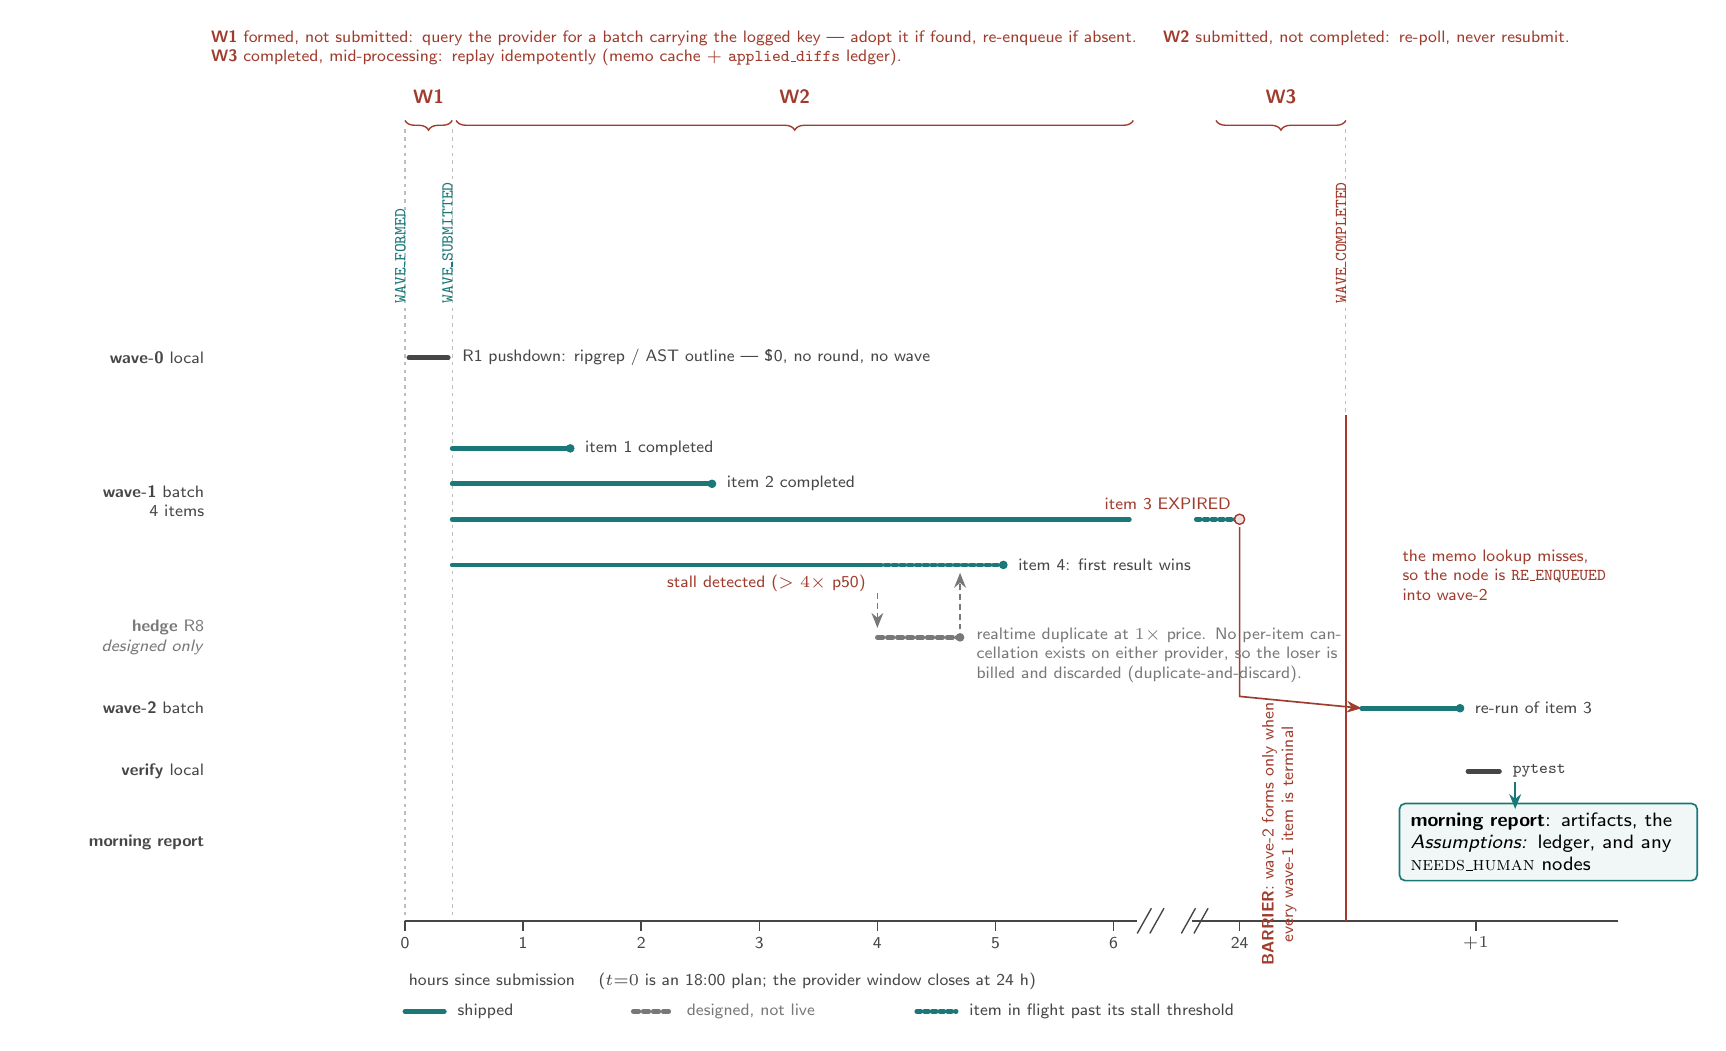
\begin{tikzpicture}[x=1cm,y=1cm]

\tikzset{
  lane/.style={lbls, anchor=east, align=right, text width=2.2cm},
  itembar/.style={draw=accent, line width=1.7pt, line cap=round},
  stallbar/.style={draw=accent, line width=1.7pt, line cap=round,
                   dash pattern=on 1.4pt off 1.4pt},
  hedgebar/.style={draw=dimmed, line width=1.7pt, line cap=round,
                   dash pattern=on 2pt off 1.6pt},
  tick/.style={draw=inkgray, line width=0.5pt},
  guide/.style={draw=inkgray!35, line width=0.4pt, dash pattern=on 1.2pt off 1.6pt},
  evt/.style={font=\sffamily\fontsize{6}{7}\selectfont, text=accent, inner sep=1pt},
  endcap/.style={circle, fill=accent, inner sep=1.1pt},
}

% ---- geometry -------------------------------------------------------------
% hours 0..6  -> x = 0 .. 9   (1.5 cm/h); break at 9.3..10.2; 24 h -> x = 10.6
\def\XEXP{10.6}\def\XEND{15.4}\def\XBAR{11.95}
\def\LEFT{-2.5}

% ---- lane geometry --------------------------------------------------------
\def\ywzero{0.55}
\def\yiA{-0.6}\def\yiB{-1.05}\def\yiC{-1.5}\def\yiD{-2.08}
\def\yhedge{-3.0}\def\ywtwo{-3.9}\def\yver{-4.7}\def\yrep{-5.6}
\def\ay{-6.6}

% ---- crash-window explanation (top) --------------------------------------
\node[lbls, text=danger, anchor=north west, align=left, text width=17.2cm] at (\LEFT,4.75)
  {\textbf{W1} formed, not submitted: query the provider for a batch carrying the logged key
   \textemdash{} adopt it if found, re-enqueue if absent. \quad
   \textbf{W2} submitted, not completed: re-poll, never resubmit. \quad
   \textbf{W3} completed, mid-processing: replay idempotently
   (memo cache $+$ \texttt{applied\_diffs} ledger).};

% ---- crash windows --------------------------------------------------------
\draw[decorate, decoration={brace, amplitude=3.5pt, raise=1pt}, draw=danger, line width=0.5pt]
  (0.6,3.6) -- (0.0,3.6) node[wtag, midway, above=3.5pt] {W1};
\draw[decorate, decoration={brace, amplitude=3.5pt, raise=1pt}, draw=danger, line width=0.5pt]
  (9.25,3.6) -- (0.65,3.6) node[wtag, midway, above=3.5pt] {W2};
\draw[decorate, decoration={brace, amplitude=3.5pt, raise=1pt}, draw=danger, line width=0.5pt]
  (\XBAR,3.6) -- (10.3,3.6) node[wtag, midway, above=3.5pt] {W3};

% ---- durable event markers ------------------------------------------------
\draw[guide] (0.0,3.45) -- (0.0,\ay);
\draw[guide] (0.6,3.45) -- (0.6,\ay);
\draw[guide] (\XBAR,3.45) -- (\XBAR,\ay);
\node[evt, rotate=90, anchor=west] at (-0.06,1.20) {\texttt{WAVE\_FORMED}};
\node[evt, rotate=90, anchor=west] at (0.54,1.20) {\texttt{WAVE\_SUBMITTED}};
\node[evt, rotate=90, anchor=west, text=danger] at (\XBAR-0.06,1.20) {\texttt{WAVE\_COMPLETED}};

% ---- axis -----------------------------------------------------------------
\draw[tick] (0,\ay) -- (9.3,\ay);
\draw[tick] (10.0,\ay) -- (\XEND,\ay);
\draw[tick] (9.30,\ay-0.16) -- (9.48,\ay+0.16);
\draw[tick] (9.46,\ay-0.16) -- (9.64,\ay+0.16);
\draw[tick] (9.86,\ay-0.16) -- (10.04,\ay+0.16);
\draw[tick] (10.02,\ay-0.16) -- (10.20,\ay+0.16);
\foreach \h in {0,1,2,3,4,5,6} {
  \draw[tick] (1.5*\h,\ay) -- (1.5*\h,\ay-0.13);
  \node[lbls, anchor=north] at (1.5*\h,\ay-0.16) {\h};
}
\draw[tick] (\XEXP,\ay) -- (\XEXP,\ay-0.13);
\node[lbls, anchor=north] at (\XEXP,\ay-0.16) {24};
\draw[tick] (13.6,\ay) -- (13.6,\ay-0.13);
\node[lbls, anchor=north] at (13.6,\ay-0.16) {$+1$};
\node[lbls, anchor=north west, align=left] at (0,\ay-0.62)
  {hours since submission \quad ($t{=}0$ is an 18:00 plan; the provider window closes at 24 h)};

% ---- lane labels ----------------------------------------------------------
\node[lane] at (\LEFT,\ywzero) {\textbf{wave-0} local};
\node[lane] at (\LEFT,\yiB-0.22) {\textbf{wave-1} batch\\ 4 items};
\node[lane, text=dimmed] at (\LEFT,\yhedge) {\textbf{hedge} R8\\ \emph{designed only}};
\node[lane] at (\LEFT,\ywtwo) {\textbf{wave-2} batch};
\node[lane] at (\LEFT,\yver) {\textbf{verify} local};
\node[lane] at (\LEFT,\yrep) {\textbf{morning report}};

% ---- wave-0 ---------------------------------------------------------------
\draw[itembar, draw=inkgray] (0.05,\ywzero) -- (0.55,\ywzero);
\node[lbls, anchor=west] at (0.68,\ywzero)
  {R1 pushdown: ripgrep / AST outline \textemdash{} \$0, no round, no wave};

% ---- wave-1 items ---------------------------------------------------------
\newcommand{\itemrow}[3]{%
  \draw[itembar] (0.6,#1) -- (#2,#1);
  \node[endcap] at (#2,#1) {};
  \node[lbls, anchor=west] at (#2+0.14,#1) {#3};}

\itemrow{\yiA}{2.1}{item 1 completed}
\itemrow{\yiB}{3.9}{item 2 completed}

% item 3: never returns, expires at the window ceiling
\draw[itembar]  (0.6,\yiC) -- (9.2,\yiC);
\draw[stallbar] (10.05,\yiC) -- (\XEXP,\yiC);
\node[circle, draw=danger, fill=danger!15, line width=0.5pt, inner sep=1.3pt] at (\XEXP,\yiC) {};
\node[lbls, anchor=south east, text=danger] at (\XEXP-0.06,\yiC+0.08) {item 3 EXPIRED};
\draw[ar, draw=danger] (\XEXP,\yiC-0.1) -- (\XEXP,\ywtwo+0.15) -- (12.15,\ywtwo);
\node[lbls, anchor=north west, align=left, text=danger, text width=3.5cm]
  at (12.62,\yiC-0.34) {the memo lookup misses,\\ so the node is
  \texttt{RE\_ENQUEUED}\\ into wave-2};

% item 4: stalls, hedge fires, first result wins
\draw[itembar]  (0.6,\yiD) -- (6.0,\yiD);
\draw[stallbar] (6.0,\yiD) -- (7.6,\yiD);
\node[endcap] at (7.6,\yiD) {};
\node[lbls, anchor=west] at (7.74,\yiD) {item 4: first result wins};
\node[lbls, anchor=north east, text=danger] at (5.9,\yiD-0.08) {stall detected ($>4\times$ p50)};
\draw[dar] (6.0,\yiD-0.36) -- (6.0,\yhedge+0.12);
\draw[hedgebar] (6.0,\yhedge) -- (7.05,\yhedge);
\node[circle, fill=dimmed, inner sep=1.1pt] at (7.05,\yhedge) {};
\draw[dar] (7.05,\yhedge+0.1) -- (7.05,\yiD-0.1);
\node[dlbl, anchor=north west, align=left, text width=4.6cm,
      font=\sffamily\fontsize{6}{7}\selectfont] at (7.2,\yhedge+0.18)
  {realtime duplicate at $1\times$ price. No per-item cancellation exists on either
   provider, so the loser is billed and discarded (duplicate-and-discard).};

% ---- barrier --------------------------------------------------------------
\draw[danger, line width=0.9pt] (\XBAR,\yiA+0.42) -- (\XBAR,\ay);
\node[lbls, text=danger, anchor=south, rotate=90, align=center] at (\XBAR-0.58,\yrep+0.1)
  {\textbf{BARRIER}: wave-2 forms only when\\ every wave-1 item is terminal};

% ---- wave-2, verify, morning report ---------------------------------------
\draw[itembar] (12.15,\ywtwo) -- (13.4,\ywtwo);
\node[endcap] at (13.4,\ywtwo) {};
\node[lbls, anchor=west] at (13.54,\ywtwo) {re-run of item 3};
\draw[itembar, draw=inkgray] (13.5,\yver) -- (13.9,\yver);
\node[lbls, anchor=west] at (14.02,\yver) {\texttt{pytest}};
\node[boxs, text width=3.5cm, anchor=west, align=left] (rep) at (12.62,\yrep)
  {\textbf{morning report}: artifacts, the \emph{Assumptions:} ledger,
   and any \textsc{needs\_human} nodes};
\draw[ar] (14.1,\yver-0.14) -- (14.1,\yrep+0.42);

% ---- legend ---------------------------------------------------------------
\def\ly{-7.75}
\draw[itembar] (0.0,\ly) -- (0.5,\ly);
\node[lbls, anchor=west] at (0.62,\ly) {shipped};
\draw[hedgebar] (2.9,\ly) -- (3.4,\ly);
\node[dlbl, anchor=west, font=\sffamily\fontsize{6}{7}\selectfont] at (3.52,\ly)
  {designed, not live};
\draw[stallbar] (6.5,\ly) -- (7.0,\ly);
\node[lbls, anchor=west] at (7.12,\ly) {item in flight past its stall threshold};

\end{tikzpicture}}

\caption{\textbf{Wave execution over a night.} Barriers separate waves; within a wave, items complete independently. The hedge path (dimmed: designed, not yet live) races a realtime duplicate against a stalled item under duplicate-and-discard semantics --- the redesign forced by the absence of per-item cancellation. Expired items re-enter the next wave through the memo check. W1--W3 are the crash windows of \cref{sec:crash}.}
\label{fig:wavetimeline}
\end{figure}

\section{Implementation truth}
\label{sec:implementation}

The system is 16{,}979 lines of Python (8{,}845 in the package, 7{,}281 in tests, 853 in the benchmark harness) with 368 tests. Three findings from auditing our own code, reported because papers rarely do and reviewers always should.

\paragraph{The optimizer is an architecture, not yet an optimizer.} The shipped rewrite layer is 200 lines implementing two rules; R2's entire rewrite is one boolean flip under a hardcoded two-file threshold, and R1 trusts a planner-supplied flag rather than analyzing answerability --- moreover its ``free local execution'' currently emits a question-and-scope artifact, not ripgrep/AST output (the operator schema has no \texttt{context\_spec} to harvest), so fan-out driven by a local \textsc{Explore} cannot yet resolve. There is no cost model, no adaptive re-optimization at wave boundaries, and \texttt{Caps}-aware splitting is validated post-hoc by adapters rather than planned around. The query-engine \emph{shape} --- typed IR, rewrite pass, physical lowering, execution --- is real and tested; the query-engine \emph{intelligence} is the roadmap. Relatedly, wave count equals DAG depth today only because a single model makes (provider, model) grouping degenerate, and the statically-computed layer assignment is discarded in favor of dynamically formed, content-addressed waves.

\paragraph{The state machine is $\sim$40\% aspirational.} Of 21 declared node states, 8 are unreachable (hedging, speculation, repair, gating, cancellation); of 23 event types, 2 are never emitted. We keep the full vocabulary in the schema deliberately --- events are append-only and renaming is a migration --- but the paper's figures dim what the runtime cannot reach.

\paragraph{Crash safety is the strongest subsystem.} Every claim in \cref{sec:crash} traces to tested code paths: the three windows each have a dedicated recovery with a dedicated test, including kill-9-mid-wave resume that adopts the orphaned provider batch rather than double-paying. Where the rest of the system is honest scaffolding, this part is load-bearing today --- which is the right inversion for an unattended-execution product.

\paragraph{Evaluation status.} A benchmark harness (three fixture tasks, a pricing model, and a Claude-Code-CLI baseline runner) ships; the only committed result is a mock-provider plumbing run. The economics of \cref{sec:economics} are therefore \emph{derived and reviewed}, not yet \emph{measured} --- the honest gap a reviewer should press on, and the immediate next step now that the companion self-hosted batch tier (Tidal, evaluated on GPU in its own paper) provides a meterable execution target: the same fixture tasks run end-to-end against self-hosted batch capacity with per-item token ledgers, alongside realized \texttt{rounds\_per\_node} and within-wave cache-hit measurements.

\section{Should this generalize? Frameworks, and an honest verdict}
\label{sec:generalization}

LazyCode is a coding CLI. The obvious question --- asked of us, and by us --- is whether plan-online/execute-on-batch belongs in general agentic frameworks: Pydantic AI with its durable-execution backends, NVIDIA's NeMo Agent Toolkit, LangGraph and kin. The answer we defend: \emph{partially, and not as an architecture}.

\paragraph{The substrate exists; the seam does not.} Durable-execution integration is a solved problem: Pydantic AI ships co-maintained DBOS, Temporal, Prefect and Restate backends behind a public capability interface, with cost-budget gating built in; DBOS alone provides exactly-once steps, checkpointed multi-day sleeps, deduplication ids (LazyCode's idempotency key, ready-made) and rate-limited queues --- and its old Postgres objection has expired (SQLite is now the default). What no framework has is a \emph{first-class batch-API abstraction for model requests}: durable backends do wrap model calls in activities/steps (and Temporal can suspend turns on durable timers), but an activity-wrapped model call still completes as one synchronous unit --- there is no protocol for terminating a run at a model call, pooling it into a provider batch, and resuming hours later from persisted history, the way Pydantic AI's deferred-\emph{tool} protocol already does for tools. The single upstream change that unblocks the entire ecosystem is a \texttt{DeferredModelRequests} analogue of the existing deferred-tools protocol --- terminate the run at a model call, resume from persisted history plus results. The transport machinery already ships; the protocol extension is small; an open issue has waited since May 2025 for exactly this design.

\paragraph{The negative control.} NeMo Agent Toolkit --- the most explicitly engineered framework in the field --- has a genuinely strong profiler (including a common-prefix detector that independently rediscovers R4 from the serving side, and latency-tier routing hints into Dynamo) yet no durable \emph{mid-run} suspension (its async job submission and SQL-backed job store are endpoint-scoped, and human-in-the-loop pauses are in-process), no cost-tier routing, an empty cron stub, and no provider-batch integration. The gap LazyCode fills is real across the ecosystem, not an artifact of coding CLIs. Meanwhile the only prior attempts at agent-side batch use are two 2026 fleet-pooling prototypes (a proxy that batches across a fleet of agents; a queue-flush router with per-call latency budgets) --- both dispatcher-level, both stopping short of barriers, memoization, deadline machinery, and crash safety. Evaluation harnesses that \emph{do} support batch APIs explicitly warn against using them for agentic tasks. The field has found the door; nobody has walked through it.

\paragraph{The criterion.} The architecture pays exactly where a workload satisfies four conditions:
\emph{(a) the environment is snapshottable} --- LazyCode pins a git commit and applies diffs into an immutable fork, so an 18:00 plan is still valid at 03:00; a CRM-writing or browser agent acts on a live world that moves during the wave, and deferred action against an unversioned environment silently invalidates its own premises;
\emph{(b) a cheap deterministic oracle exists} --- pytest and compilers make \textsc{Verify} free and local; where the only verifier is an LLM judge, failure is discovered a wave late and the repair round erases the discount;
\emph{(c) width dominates depth} --- structurally within the task, or by inter-run concurrency (\cref{sec:economics-width});
\emph{(d) laxity is positive} --- nobody is waiting.
Coding is the canonical member of this class --- versioned by git, oracled by test suites, fan-out-able by file --- but it is a member, not the definition. Repo-scale migrations, IaC changes (\texttt{terraform plan} as oracle), corpus extraction under schema contracts, and evaluation/synthetic-data fleets all qualify. Interactive copilots, SLA-bound triage, and live-environment actuation never will; naming that boundary is a contribution, because a naive generalization into those classes would do real damage.

% FIGURE 6 SPEC (fig-quadrant.tex): 2x2-ish decision chart. X axis: "environment snapshottable +
% cheap oracle" (no -> yes). Y axis: "width available / laxity" (low -> high). Place labeled dots:
% top-right (accent, "pays"): repo migrations, test coverage, corpus extraction w/ schema, eval fleets,
% IaC (terraform plan); bottom-right: one-off deep code tasks ("use interactive");
% top-left (red-ish, "never"): browser/computer-use fleets, CRM writers; bottom-left: copilots,
% support agents, incident response. Annotate the four-part criterion (a)-(d) beside axes.
\begin{figure}[!htbp]
\centering
% Figure 6 -- where plan-online / execute-on-batch pays: the four-part criterion as a map.
\resizebox{\linewidth}{!}{%
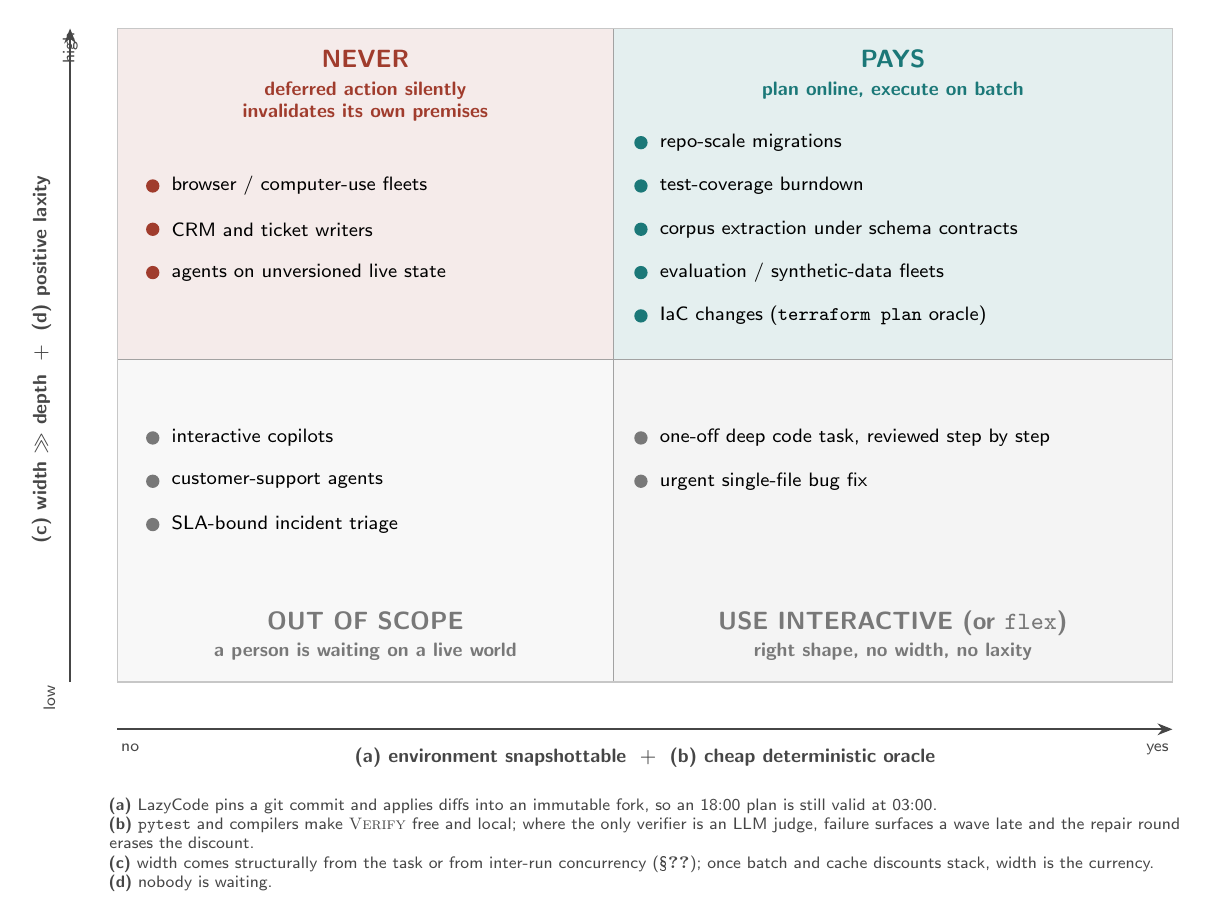
\begin{tikzpicture}[x=1cm,y=1cm]

\tikzset{
  dot/.style={circle, fill=accent, inner sep=1.7pt},
  ddot/.style={circle, fill=danger, inner sep=1.7pt},
  gdot/.style={circle, fill=dimmed, inner sep=1.7pt},
  pt/.style={font=\sffamily\scriptsize, text=black, inner sep=1.5pt, align=left},
  qhead/.style={font=\sffamily\bfseries\small, align=center},
}
\newcommand{\qsub}[1]{{\sffamily\fontsize{6.8}{8}\selectfont #1}}

\def\XL{0}\def\XM{6.3}\def\XR{13.4}
\def\YB{0}\def\YM{4.1}\def\YT{8.3}

% ---- quadrant fills -------------------------------------------------------
\fill[accent!12]  (\XM,\YM) rectangle (\XR,\YT);
\fill[danger!10]  (\XL,\YM) rectangle (\XM,\YT);
\fill[dimmed!8]   (\XM,\YB) rectangle (\XR,\YM);
\fill[dimmed!5]   (\XL,\YB) rectangle (\XM,\YM);

\draw[inkgray!50, line width=0.5pt] (\XL,\YM) -- (\XR,\YM);
\draw[inkgray!50, line width=0.5pt] (\XM,\YB) -- (\XM,\YT);
\draw[inkgray!30, line width=0.5pt] (\XL,\YB) rectangle (\XR,\YT);

% ---- quadrant headings ----------------------------------------------------
\node[qhead, text=accent, anchor=north] at (9.85,\YT-0.15)
  {PAYS \\[-1pt] \qsub{plan online, execute on batch}};
\node[qhead, text=danger, anchor=north] at (3.15,\YT-0.15)
  {NEVER \\[-1pt] \qsub{deferred action silently} \\[-3pt]
   \qsub{invalidates its own premises}};
\node[qhead, text=dimmed, anchor=south] at (9.85,\YB+0.15)
  {USE INTERACTIVE (or \texttt{flex}) \\[-1pt] \qsub{right shape, no width, no laxity}};
\node[qhead, text=dimmed, anchor=south] at (3.15,\YB+0.15)
  {OUT OF SCOPE \\[-1pt] \qsub{a person is waiting on a live world}};

\newcommand{\mk}[4]{\node[#4] (p#1) at (#2) {}; \node[pt, anchor=west] at ($(#2)+(0.18,0)$) {#3};}

% ---- upper right: pays ----------------------------------------------------
\mk{a}{6.65,6.85}{repo-scale migrations}{dot}
\mk{b}{6.65,6.30}{test-coverage burndown}{dot}
\mk{c}{6.65,5.75}{corpus extraction under schema contracts}{dot}
\mk{d}{6.65,5.20}{evaluation / synthetic-data fleets}{dot}
\mk{e}{6.65,4.65}{IaC changes (\texttt{terraform plan} oracle)}{dot}

% ---- lower right ----------------------------------------------------------
\mk{f}{6.65,3.10}{one-off deep code task, reviewed step by step}{gdot}
\mk{g}{6.65,2.55}{urgent single-file bug fix}{gdot}

% ---- upper left -----------------------------------------------------------
\mk{h}{0.45,6.30}{browser / computer-use fleets}{ddot}
\mk{i}{0.45,5.75}{CRM and ticket writers}{ddot}
\mk{j}{0.45,5.20}{agents on unversioned live state}{ddot}

% ---- lower left -----------------------------------------------------------
\mk{k}{0.45,3.10}{interactive copilots}{gdot}
\mk{l}{0.45,2.55}{customer-support agents}{gdot}
\mk{m}{0.45,2.00}{SLA-bound incident triage}{gdot}

% ---- axes -----------------------------------------------------------------
\draw[arg] (\XL,-0.6) -- (\XR,-0.6);
\node[lbls, anchor=north west] at (\XL,-0.74) {no};
\node[lbls, anchor=north east] at (\XR,-0.74) {yes};
\node[lbl, anchor=north] at (6.7,-0.78)
  {\textbf{(a) environment snapshottable} $\;+\;$ \textbf{(b) cheap deterministic oracle}};

\draw[arg] (-0.6,\YB) -- (-0.6,\YT);
\node[lbls, anchor=south east, rotate=90] at (-0.74,\YB) {low};
\node[lbls, anchor=north east, rotate=90] at (-0.74,\YT) {high};
\node[lbl, anchor=south, rotate=90] at (-0.78,\YM)
  {\textbf{(c) width $\gg$ depth} $\;+\;$ \textbf{(d) positive laxity}};

% ---- criterion notes ------------------------------------------------------
\node[lbls, anchor=north, align=left, text width=13.6cm] at (6.7,-1.42)
  {\textbf{(a)} LazyCode pins a git commit and applies diffs into an immutable fork, so an
   18:00 plan is still valid at 03:00.\\
   \textbf{(b)} \texttt{pytest} and compilers make \textsc{Verify} free and local; where the
   only verifier is an LLM judge, failure surfaces a wave late and the repair round erases
   the discount.\\
   \textbf{(c)} width comes structurally from the task or from inter-run concurrency
   (\S\ref{sec:economics-width}); once batch and cache discounts stack, width is the
   currency.\\
   \textbf{(d)} nobody is waiting.};

\end{tikzpicture}}

\caption{\textbf{Where plan-online/execute-on-batch pays.} The four-part criterion as a map. The architecture's home turf is the upper right; the upper left is the danger zone where deferred execution silently invalidates its own premises.}
\label{fig:quadrant}
\end{figure}

\paragraph{Transfer analysis and verdict.} Component by component: the \emph{wave executor} --- barrier scheduling reinterpreted over $N$ concurrent runs, memoization (R10 verbatim), prefix factoring (R4, now more valuable under discount stacking), vectorization plumbing (R6), laxity-driven \{sync, flex, batch\} routing with duplicate-and-discard hedging (R8), and the assumption ledger --- transfers cleanly and is worth building as a $\sim$1--2k-line framework-agnostic library with thin DBOS/Temporal recipes and a Pydantic AI capability for cross-run pooling. The \emph{planner, operator algebra, and code-analysis rules} (R1--R3, R9, the harvester) do not transfer: their content is ripgrep, per-file independence, and free test oracles --- irreducibly coding. Our recommendation, in ascending order of leverage: build the library; ship the pooling capability; and above all land the deferred-model-request protocol upstream, because it is small, it is the true blocker, and it converts every durable-execution framework into a potential batch citizen at once.

\section{Related work}
\label{sec:related}

\emph{Semantic operators and LLM query optimization.} LOTUS, Palimpzest, Abacus, DocETL and Aryn establish cost-based optimization over declarative LLM pipelines; they own the operator-DAG-with-optimizer idea for \emph{data} processing. LazyCode's distinction is the workload class --- stateful, side-effecting, tool-using engineering work against a versioned environment with contract verification --- and the batch-API execution substrate. \emph{Model routing}: FrugalGPT and RouteLLM give the cost-tiering lineage for R5; the verify-pass-rate-gated variant is ours but unimplemented. \emph{Agent-DAG serving}: Halo and Helium consolidate multi-agent queries into optimized DAGs with KV-sharing on \emph{local} serving --- the same instincts, the opposite deployment; sleep-time compute is adjacent (idle-time precomputation, not deferred pricing). \emph{Coding agents}: SWE-agent's measured trajectory depths ($\approx$13--15 turns) calibrate what $T$ the economics condition must beat. \emph{Batch tooling}: Curator, Ray Data LLM, and evaluation harnesses batch \emph{independent} calls; none run an agentic loop through the batch tier, and the leading eval framework warns against trying. \emph{Fleet pooling}: two 2026 prototypes mark independent convergence on inter-run batching, minus the systems machinery. \emph{Database lineage}: the transplant's ancestors are explicit --- System~R's cost-based optimization, Volcano/Cascades rewrite architecture, ARIES-style write-ahead recovery, and Saga-style compensation for long-lived transactions --- and the paper's claim is the transplant, not the machinery. \emph{Coding agents beyond SWE-agent}: OpenHands, Aider, and Agentless calibrate the interactive baseline space. \emph{Serving side}: the companion Tidal paper supplies the self-hosted batch tier (deadline-contracted co-serving on vLLM) that closes the loop this paper's adapter opens. The unoccupied conjunction LazyCode claims: a barrier-scheduled, memoized, crash-safe, deadline-aware batch executor driving a stateful, contract-verified agent against a snapshottable environment.

\section{Limitations}
\label{sec:limitations}

The economics are derived, not yet measured: no real-provider benchmark run exists, realized \texttt{rounds\_per\_node} is uninstrumented (the current counter can only report 1), and within-wave cache hit rates --- on which \cref{sec:economics-width} leans --- are best-effort and unbooked. Provider latency tails are unpublished; the overnight guarantee is ``most nights, with a priced fallback,'' not an SLA, and a hedge that fires re-buys realtime pricing for that item. The optimizer intelligence, hedging, repair, model tiering, vectorization $k{>}1$, and per-item cost accounting are designed but not live; the state machine carries their vocabulary ahead of their arrival. The flex tier undercuts the pure-discount motivation on one provider today. Three code-level debts surfaced by review: the adapter requests the default 5-minute cache TTL rather than the 1-hour TTL the width economics assume; Anthropic-side batch-metadata round-tripping (on which orphan adoption rests) is unverified against the live API; and local \textsc{Explore} produces a scope stub rather than tool output. And the architecture's preconditions --- git-snapshottable state, free oracles --- bound its domain honestly: this is a compiler for a particular, valuable shape of work, not a universal agent runtime.

\section{Conclusion}

Data systems learned to go from batch to streaming; LazyCode runs the lesson in reverse for agents, and finds the pieces already lying around: a planning model that can emit typed DAGs, providers selling half-price deferred execution, database machinery for making it crash-safe, and --- newly quantified here --- discount stacking that rewards width more than heroic depth-collapse. The system's honest state is a strong skeleton with two shipped rewrite rules, bulletproof recovery, and unmeasured economics; its honest future is a measurement campaign against its companion self-hosted batch tier, and a small upstream protocol change that would let every agent framework defer a model call. The compiler metaphor sets the standard the project must ultimately meet: not that batch execution is architecturally workable --- the shipped machinery and its crash-safety argue that much --- but that the compilation is profitable, case by case, with the receipts to show it.

\section*{Acknowledgments}
The design benefited from adversarial multi-model review; several of this paper's central corrections (the cached-baseline economics, the vacant-speculation example, the width-dependent refinement) were surfaced by reviews that set out to break the claims rather than confirm them.

\begin{thebibliography}{30}\small
\bibitem{lotus} L.~Patel et al. LOTUS: Semantic Operators for Bulk LLM Processing. VLDB 2025. arXiv:2407.11418.
\bibitem{palimpzest} C.~Liu, M.~Russo, M.~Cafarella et al. Palimpzest: Optimizing AI-Powered Analytics. CIDR 2025. arXiv:2405.14696.
\bibitem{abacus} Abacus: Cost-Based Optimization for Semantic Operator Systems. arXiv:2505.14661.
\bibitem{docetl} S.~Shankar et al. DocETL: Agentic Query Rewriting for Complex Document Processing. arXiv:2410.12189.
\bibitem{frugalgpt} L.~Chen, M.~Zaharia, J.~Zou. FrugalGPT. arXiv:2305.05176.
\bibitem{routellm} I.~Ong et al. RouteLLM: Learning to Route LLMs. arXiv:2406.18665.
\bibitem{halo} Halo: Holistic Agent-DAG Optimization for LLM Serving. arXiv:2509.02121.
\bibitem{helium} Helium: DAG-Consolidated Serving for Agentic Workflows. arXiv:2603.16104.
\bibitem{sleeptime} K.~Lin et al. Sleep-time Compute. arXiv:2504.13171.
\bibitem{sweagent} J.~Yang et al. SWE-agent: Agent-Computer Interfaces Enable Automated Software Engineering. arXiv:2405.15793.
\bibitem{tidal} G.~Lunkupali Venugopal. Tidal: An SLA-Contracted Batch Tier for LLM Serving Engines. 2026. github.com/rajagurunath/tidal.
\bibitem{pydanticai} Pydantic AI: Durable Execution (DBOS, Temporal, Prefect, Restate). pydantic.dev/docs/ai, 2026.
\bibitem{dbos} DBOS: Durable Workflows. docs.dbos.dev, 2026.
\bibitem{nat} NVIDIA NeMo Agent Toolkit (v1.8). github.com/NVIDIA/NeMo-Agent-Toolkit, 2026.
\bibitem{inspect} UK AISI. Inspect AI: Batch Mode. inspect.aisi.org.uk/models-batch.html.
\bibitem{anthropic-batch} Anthropic. Message Batches and Prompt Caching documentation. platform.claude.com/docs, 2026.
\bibitem{openai-batch} OpenAI. Batch API, Flex Processing, and Webhooks documentation. developers.openai.com, 2026.
\bibitem{fleetblog} E.~Sandler. Batch API is terrible for one agent. It might be great for a fleet. Apr 2026. github.com/erans/batching-harness.
\bibitem{llmfleet} llmfleet: latency-budget routing to batched Anthropic calls. github.com/MukundaKatta/llmfleet, 2026.
\bibitem{curator} Bespoke Labs. Curator. github.com/bespokelabsai/curator.
\bibitem{volcano} G.~Graefe. Volcano --- An Extensible and Parallel Query Evaluation System. IEEE TKDE, 1994.
\bibitem{selinger} P.~G.~Selinger et al. Access Path Selection in a Relational DBMS. SIGMOD 1979.
\bibitem{cascades} G.~Graefe. The Cascades Framework for Query Optimization. IEEE Data Eng.\ Bull., 1995.
\bibitem{aries} C.~Mohan et al. ARIES: A Transaction Recovery Method. ACM TODS, 1992.
\bibitem{sagas} H.~Garcia-Molina, K.~Salem. Sagas. SIGMOD 1987.
\bibitem{openhands} X.~Wang et al. OpenHands: An Open Platform for AI Software Developers. arXiv:2407.16741.
\bibitem{agentless} C.~Xia et al. Agentless: Demystifying LLM-based Software Engineering Agents. arXiv:2407.01489.
\bibitem{spark-aqe} Apache Spark: Adaptive Query Execution. spark.apache.org.
\end{thebibliography}

\end{document}
